\special{pdf:minorversion 7}
\PassOptionsToPackage{dvipsnames}{xcolor}
\documentclass[11pt,a4paper]{report}

\usepackage[todonotes={textsize=scriptsize}, draft]{changes}
\usepackage[left=3cm, right=3cm, top=3cm, bottom=3.5cm]{geometry}
\usepackage{setspace}
\usepackage{layout}
\usepackage{parskip}
\usepackage{amsmath}
\usepackage{amssymb}
\usepackage[T1]{fontenc}
\usepackage{fontspec}
\setmainfont{XCharter}
\usepackage{unicode-math}
\setmathfont{XCharter-Math.otf}
\setsansfont{IBMPlexSans}[
    Extension = .otf,
    UprightFont = *-Regular,
    BoldFont = *-SemiBold,
    ItalicFont = *-Italic,
    BoldItalicFont = *-SemiBoldItalic,
    Scale = MatchLowercase
]
\setmonofont{IBMPlexMono}[Scale=MatchLowercase]
\usepackage{multicol}
\usepackage{multirow}
\usepackage{pdfpages}
\usepackage{pdflscape}
\usepackage{graphicx}
% \DeclareGraphicsExtensions{.png,.pdf}
\DeclareGraphicsExtensions{.pdf,.png}
\usepackage{tabularx}
% \usepackage{expl3}
% \usepackage{calc}
\usepackage[version=4]{mhchem}
\usepackage{siunitx}
\usepackage{bm}
\usepackage[dvipsnames]{xcolor}
\usepackage{caption}
\usepackage{subcaption}
\usepackage[sf,bf]{titlesec}
\usepackage{colortbl}
\usepackage{enumitem}
\usepackage{listings}
\usepackage{booktabs}
\usepackage{gensymb}
\usepackage[font=itshape]{quoting}
\usepackage{wrapfig}
\usepackage{fancyhdr}
\usepackage{lipsum}
\usepackage{draftwatermark}
\usepackage{soul}
\usepackage[
    style=ieee,
    citestyle=numeric-comp,
    urldate=iso]{biblatex}
% \usepackage{datetime}
\usepackage{nameref}
\usepackage{hyperref}
\definecolor{McGillRed}{cmyk}{0, 1, 0.9, 0}
\hypersetup{
    colorlinks=true,
    linkcolor=cyan,
    anchorcolor=cyan,
    citecolor=cyan,
    filecolor=cyan,
    urlcolor=cyan
}
\setdeletedmarkup{\textcolor{McGillRed}{\sout{#1}}}
\definechangesauthor[color=violet, name={Emmanuel Duplay}]{ED}
\definechangesauthor[color=cyan, name={Barry Zandbergen}]{BZ}
\definechangesauthor[color=McGillRed, name={Andrew Higgins}]{AH}

% \input{titlesec.tex}
\addbibresource{ref.bib}

\title{Design and Test of a laser-plasma thruster laboratory model}
\author{Emmanuel Duplay}
\date{0000-00-00}

\renewcommand{\headrulewidth}{0pt}
\renewcommand{\chaptermark}[1]{\markboth{\MakeUppercase{\thechapter.\ #1}}{}}
\renewcommand{\sectionmark}[1]{\markright{\MakeUppercase{\thesection.\ #1}}}

\renewcommand{\chapterautorefname}{Chapter}
\renewcommand{\sectionautorefname}{Section}

\newcommand{\shotsettings}[4]{\texttt{#1}: #2~ms, \textit{f}/#3, ND#4}

\newcommand{\dd}[2]{\frac{\mathrm{d}#1}{\mathrm{d}#2}}
\newcommand{\ddi}[2]{\mathrm{d}#1/\mathrm{d}#2}

% Track changes commands
% \newcommand{\change}[1]{\textcolor{McGillRed}{#1}}
% \newenvironment{changeblock}{\color{McGillRed}}{}
% \renewcommand{\change}[1]{#1}  % Comment out to suppress changes
% \renewenvironment{changeblock}{}{}  % Comment out to suppress changes

\fancypagestyle{fancy}{
    \fancyhf{}
    \fancyhfinit{\sffamily}
    \lhead{\leftmark}
    \rhead{\rightmark}
    \lfoot{AE5050}
    \rfoot{\thepage}
}

\fancypagestyle{plain}{
    \fancyhf{}
    \fancyfoot[C]{\sffamily \thepage}
    
}

\pagestyle{fancy}

\SetWatermarkText{\sffamily \textbf{DRAFT}}
\SetWatermarkFontSize{2cm}
\SetWatermarkColor[gray]{0.85}
    
\definecolor{bggray}{gray}{0.97}
\definecolor{txtgray}{gray}{0.3}

\lstdefinestyle{mystyle}{
    backgroundcolor=\color{bggray},   
    commentstyle=\color{MidnightBlue},
    keywordstyle=\color{Plum},
    numberstyle=\scriptsize\ttfamily\color{Gray},
    stringstyle=\color{RedOrange},
    % identifierstyle=\color{Turquoise},
    basicstyle=\ttfamily\color{txtgray},
    breakatwhitespace=false,         
    breaklines=true,                 
    captionpos=t,                    
    keepspaces=true,                 
    numbers=left,                    
    numbersep=5pt,                  
    showspaces=false,                
    showstringspaces=false,
    showtabs=false,                  
    tabsize=2
}

\lstset{style=mystyle}
\newenvironment{plainchp}[1]
    {
        \newgeometry{left=4.2cm,right=4.2cm}
        \fancypagestyle{abstractplain}{
            \fancyhf{}
            \fancyfootoffset[lh]{0pt}
            \fancyfoot[C]{\sffamily \thepage}  
        }
        \pagestyle{abstractplain}
        
        \phantomsection
        \begin{center}
            \sffamily \Large \caps{\textbf{\MakeUppercase{#1}}}
        \end{center}
        \vspace{0.2cm}
        \markboth{\MakeUppercase{#1}}{}
    }
    {
        \restoregeometry
        \pagestyle{fancy}
    }

\newenvironment{statement}[1]
    {
        \begin{center}\begin{minipage}{0.85\textwidth}
            {\sffamily \footnotesize \color{cyan}\caps{\MakeUppercase{#1}}}\\\itshape
    }
    {
        \end{minipage}\end{center}
    }

\sisetup{detect-all}

\begin{document}
    \setlength{\parindent}{0pt}
    \setlength{\headheight}{13.6pt}
    \includepdf{assets/cover.pdf}
    \begin{titlepage}
    \thispagestyle{empty}
    % \centering
    \sffamily
    \vspace*{3cm}
    {\large \color{cyan}
        % Suptitle
        Master's Thesis
    }

    \vspace{0.3cm}
    {\LARGE \textbf{Argon Laser-Plasma Thruster}}

    {\Large Design and Test of a Laboratory Model}

    \vspace{0.2cm}
    {\large 
        % Subtitle
        Submitted to fulfill the requirements of the degree of Master of Science at\\the Delft University of Technology

        \vspace{1cm}
        Emmanuel Duplay\\
        5468515 \\
        MSc. Aerospace Engineering \\
        Space Track \\
        Space Exploration Profile

        \vspace{0.5cm}
        \today
    }
    \vfill
    {   
        The work in this thesis was performed in part at the Mechanical Engineering Department of McGill University, in Montreal, Canada.
        
        \setlength{\tabcolsep}{0pt}
        \begin{tabular}{l@{:\hspace{1em}}p{0.3\textwidth}p{0.4\textwidth}}
            Internal supervisor &   Ir. B.T.C. Zandbergen & Delft University of Technology \\
            External supervisor &   Prof. A.J. Higgins & McGill University \\
            % DON'T FORGET TO REPLACE THESE PLACEHOLDERS LMAO
            Thesis committee    &   Prof. A. Menicucci 
                        \newline    Prof. A. Cervone
                                &   Delft University of Technology
                        \newline    Delft University of Technology \\
        \end{tabular}
    }
    \vspace{0.5cm}
    \begin{center}
        \includegraphics[height=1.75cm]{assets/TUDelft_logo.pdf}
        \hfill
        \includegraphics[height=1.75cm]{assets/McGill_logo.pdf}
    \end{center}
    \pagenumbering{gobble}        
\end{titlepage}

    \newpage
    % \layout*
    {   \sffamily
        \thispagestyle{empty}
        \vspace*{\fill}
        % Text width: \the\textwidth  \\ % DELETE THIS LINE BEFORE SUBMITTING
        % Text height: \the\textheight  % DELETE THIS LINE BEFORE SUBMITTING

        The code used for this project (including the \LaTeX\hspace{0.67ex}source) is available on \\ \url{https://github.com/eeduplay/MScThesis} (latest) \\ \url{https://doi.org/10.1234/0000-00000-000} (archive)

        All experimental data associated with this thesis are available on \\
        \url{https://doi.org/10.1234/0000-00000-000}\\
        This includes the list of LSPs, high-speed footage, pressure data, and spectrograms.

        The author can be contacted by email at \href{mailto:emmanuel.duplay@gmail.com}{emmanuel.duplay@gmail.com}

        Cover image: Composite photograph approximating (with some artistic license) the appearance of the laser-thermal thruster model operating in the laboratory.
    }
    \pagenumbering{roman}

    % \newgeometry{left=4.2cm,right=4.2cm}
% \fancypagestyle{abstractplain}{
%     \fancyhf{}
%     \fancyfootoffset[lh]{0pt}
%     \fancyfoot[C]{\sffamily \thepage}  
% }
% \pagestyle{abstractplain}

% \phantomsection
% \begin{center}
%     \sffamily \Large \textbf{\caps{PREFACE}}
% \end{center}
%     \addcontentsline{toc}{chapter}{Preface}
%     \markboth{\MakeUppercase{Preface}}{}
%     \label{chp:preface}
%     \vspace{0.2cm}
%     This report documents the work done during my three month internship at the Princeton Plasma Physics Laboratory (PPPL). This project stems from a collaboration between McGill University and the PPPL, following the publication of \citetitle*{duplay_design_2022}, a mission design paper I worked on while finishing my undergraduate studies at McGill. This opportunity to collaborate arose about a month before the start of the summer, as I was still struggling to find an internship, so I would like to thank my former supervisor Andrew Higgins for arranging this experience. I would also like to thank Zhuofan Bao and Paria Makaremi-Esfarjani for their assistance with parts of this project. Finally, thanks to Ahmed Diallo, my supervisor at the PPPL, for inviting me to the PPPL and being a wonderful host.

% \restoregeometry
% \pagestyle{fancy}

\begin{plainchp}{Preface}
    \addcontentsline{toc}{chapter}{Preface}
    This report documents the work done during my three month internship at the Princeton Plasma Physics Laboratory (PPPL). This project stems from a collaboration between McGill University and the PPPL, following the publication of \citetitle*{duplay_design_2022}, a mission design paper I worked on while finishing my undergraduate studies at McGill. This opportunity to collaborate arose about a month before the start of the summer, as I was still struggling to find an internship, so I would like to thank my former supervisor Andrew Higgins for arranging this experience. I would also like to thank Zhuofan Bao and Paria Makaremi-Esfarjani for their assistance with parts of this project. Finally, thanks to Ahmed Diallo, my supervisor at the PPPL, for inviting me to the PPPL and being a wonderful host.
\end{plainchp}
    \hypersetup{linkcolor=black}
    \tableofcontents
    
    \listoffigures
    \addcontentsline{toc}{chapter}{List of Figures}
    
    \listoftables
    \addcontentsline{toc}{chapter}{List of Tables}
    \hypersetup{linkcolor=cyan}
    
    \chapter*{Nomenclature}
\setlength{\columnsep}{1cm}
\newenvironment{nomtable}
    {
        \centering
        \tabularx{\columnwidth}{r>{\raggedright\arraybackslash}X}
    }
    {
        \endtabularx
    }
\newenvironment{nomlist}
    {
        \begin{itemize}[leftmargin=1.5cm]
            \raggedright
            \setlength{\parsep}{0pt}
            \setlength{\itemsep}{-4pt}
    }
    {
        \end{itemize}
    }
\addcontentsline{toc}{chapter}{Nomenclature}
\markboth{\MakeUppercase{Nomenclature}}{}
\begin{multicols}{2}
    % \setlength{\columnseprule}{1pt}
    \section*{Abbreviations}

    \begin{nomlist}
        \item[DEP]              Directed-Energy Propulsion
        \item[FDL]              (McGill) Fluid Dynamics Laboratory
        \item[IB]               Inverse Bremsstrahlung 
        \item[IFERG]            Interstellar Flight Experimental Research Group
        \item[LSP]              Laser-Sustained Plasma
        \item[LTP]              Laser-Thermal Propulsion
        \item[LTTLM]            Laser-Thermal Thruster Laboratory Model
        \item[OTS]              Off-The-Shelf
        \item[TTL]              Transistor-to-Transistor Logic
    \end{nomlist}

    \section*{Latin symbols}
    \begin{nomlist}
        \item[$A$]              Probability of atomic energy transition [\unit{s^{-1}}]
        \item[$\mathsf{A}$]     Empirically derived parameter A for Paschen's law 
        \item[$\mathsf{B}$]     Empirically derived parameter B for Paschen's law 
        \item[$c$]              Speed of light in a vacuum (\qty{2.99792e8}{m.s^{-1}}) 
        \item[$c_p$]            Specific heat of enthalpy
        \item[$c_V$]            Specific heat of internal energy
        \item[$D$]              Diameter
        \item[$d$]              Distance
        \item[$E$]              Energy
        \item[$e$]              Elementary charge (\qty{1.60218e-19}{C})
        \item[$g$]              Degeneracy of atomic energy level
        \item[$g_0$]            Standard gravity (\qty{9.80665}{m.s^{-2}}) 
        \item[$h$]              Enthalpy
        \item[$\hbar$]          Reduced Planck constant (\qty{1.05457e-34}{J.s})
        \item[$I$]              Local laser flux [\unit{W.m^{-2}}]
        \item[$I_\text{sp}$]    Specific impulse [\unit{s}]
        \item[$k_\mathrm{B}$]   Boltzmann constant (\qty{1.38065e-23}{J.K^{-1}})
        \item[$L$]              Leak rate
        \item[$\ell$]           Relative power loss
        \item[$m$]              Mass
        \item[$\mathcal{M}$]    Molar mass
        \item[$N$]              Number of moles 
        \item[$N_\mathrm{A}$]   Avogadro's number (\qty{6.02214e+23}{mol^{-1}})
        \item[$n$]              Number density 
        \item[$n_\mathrm{sp}$]  Laser setpoint 
        \item[$P$]              Power 
        \item[$p$]              Pressure
        \item[$q$]              Charge
        \item[$R_\mathrm{g}$]   Specific gas constant
        \item[$R_\mathrm{u}$]   Universal gas constant (\qty{8.31446}{J.K^{-1}.mol^{-1}})
        \item[$T$]              Temperature
        \item[$t$]              Time
        \item[$V$]              Volume
        \item[$V_\mathrm{B}$]   Breakdown Voltage
        \item[$v$]              Velocity
        \item[$Z$]              Ion charge state
        \item[$\mathcal{Z}$]    Partition function
    \end{nomlist}

    \section*{Greek symbols}
    \begin{nomlist}
        \item[$\alpha$]         Radiation absorption coefficient [\unit{m^{-1}}]
        \item[$\gamma$]         Specific heat ratio
        \item[$\gamma_\mathrm{se}$]         Secondary-electron-emission coefficient
        \item[$\epsilon$]       Integrated line emission intensity 
        \item[$\epsilon_0$]     Permittivity of free space (\qty{8.85419e-12}{F.m^{-1}})
        \item[$\Lambda_\mathrm{th}$]        Thermal DeBroglie wavelength
        \item[$\lambda$]        Wavelength
        \item[$\nu$]            Frequency
        \item[$\rho$]           Density
        \item[$\rho_\mathrm{min}$]  Electron-ion collision minimum impact parameter
    \end{nomlist}

    \section*{Subscripts}
    \begin{nomlist}
        \item[c]                Thrust chamber
        \item[e]                Electron
        \item[ex]               Exhaust
        \item[f]                Focusing length
        \item[$i$]              Lower atomic energy level 
        \item[ion]              Ionization
        \item[$k$]              Upper atomic energy level 
        \item[l]                Lens
        \item[m]                Measured
        \item[r]                Laser receiver, or reference
        \item[w]                Window
    \end{nomlist}

    % \section*{Superscripts}
    % \begin{nomlist}
    %     \item[$n$]  time index
    % \end{nomlist}

\end{multicols}

    \newpage
    % \newgeometry{left=4.2cm,right=4.2cm}
% \pagestyle{abstractplain}
% \phantomsection
% \begin{center}
%     \sffamily \Large \textbf{\caps{EXECUTIVE SUMMARY}}
% \end{center}
% \markboth{Executive Summary}{}
% \addcontentsline{toc}{chapter}{Executive Summary}

% \vspace{0.2cm}
% The aim of this internship at the Princeton Plasma Physics Laboratory was to develop a transient numerical simulation of a laser-supported plasma (LSP), the core physical process powering laser-thermal pro\-pulsion (LTP), a concept that shows promise as a high thrust, high specific impulse propulsion system. This numerical solver was needed to support simulation work done at McGill University in Montreal, which provided inconclusive results on the temperature profile of a theoretical LTP thruster. Development of a transient simulation was believed to help troubleshoot the original simulation, along with potentially providing insight on several unsteady LSP phenomena. A secondary aim of this project was to lay the groundwork for constructing an experimental LTP facility to validate the results of the numerical simulations.

% A literature study on LSP experiment was first performed to gain a better understanding of the process, catalogue common experimental techniques used in the field, and identify any research gaps. Special attention was given to the types of lasers used, working gases, and ignition methods. Past facilities with significant research output were identified to eventually replicate their experimental methods.

% Development on the LSP solver then began with re-deriving existing governing equations for unsteady, axisymmetric flow, yielding a system of 3 partial-differential equations and an equation of state, similar to the Euler fluid equations, to be solved by the simulation. Conductive heat-transfer and gas-dynamics test problems were first solved numerically to practice the implementation of relevant finite-difference methods, namely FTCS and MacCormack al\-gorithms. This was followed by the implementation of the LSP solver itself in MATLAB, to make use of several components relating to laser absorption and thermodynamic properties already implemented and tested in a steady-state LSP solver, reducing development time. A modular code base inspired by the TU Delft Astrodynamics Toolbox design was selected to allow for future use and expansion of the code for further studies. Laser modelling proved to be a significant challenge as accurate physical models required complex implementation. The modular architecture of the simulator was found to be useful in integrating the various components of the code together.

% The experimental design of a new LTP facility benefitted greatly from the literature review, as critical optical elements and LSP ignition systems could be identified. Brainstorming of relevant research questions informed the selection of some diagnostics apparatus. This review of the current experimental state-of-the-art, along with the expertise of the PPPL on laser-plasma interaction, has provided confidence in the existence in research gaps and the feasibility of an experiment. Major progress was made on the implementation of the LSP simulation, with samples of the programming interface given in this report. Although issues with the chosen numerical algorithms continued to delay development past the end of the internship period, this project provided an excellent CFD learning experience, and the design of the code base will ensure a smooth continuation of the project in the future.

% Recommendations on further work for this project are given. The numerical solver is still to be completed with working numerical methods for the 1D and 2D case, along with physically realistic boundary conditions. Improvements to the solver would likely include a raytraced laser absorption model, and the decoupling of fluid dynamics physical model from the numerical solver. The design of an experimental LTP facility should move forward, informed by the literature study completed in this report, using a systems engineering approach to define experimental needs and requirements.

% \restoregeometry
% \pagestyle{fancy}

\begin{plainchp}{Executive Summary}
    \addcontentsline{toc}{chapter}{Executive Summary}

    The aim of this internship at the Princeton Plasma Physics Laboratory was to develop a transient numerical simulation of a laser-supported plasma (LSP), the core physical process powering laser-thermal pro\-pulsion (LTP), a concept that shows promise as a high thrust, high specific impulse propulsion system. This numerical solver was needed to support simulation work done at McGill University in Montreal, which provided inconclusive results on the temperature profile of a theoretical LTP thruster. Development of a transient simulation was believed to help troubleshoot the original simulation, along with potentially providing insight on several unsteady LSP phenomena. A secondary aim of this project was to lay the groundwork for constructing an experimental LTP facility to validate the results of the numerical simulations.

    A literature study on LSP experiment was first performed to gain a better understanding of the process, catalogue common experimental techniques used in the field, and identify any research gaps. Special attention was given to the types of lasers used, working gases, and ignition methods. Past facilities with significant research output were identified to eventually replicate their experimental methods.

    Development on the LSP solver then began with re-deriving existing governing equations for unsteady, axisymmetric flow, yielding a system of 3 partial-differential equations and an equation of state, similar to the Euler fluid equations, to be solved by the simulation. Conductive heat-transfer and gas-dynamics test problems were first solved numerically to practice the implementation of relevant finite-difference methods, namely FTCS and MacCormack al\-gorithms. This was followed by the implementation of the LSP solver itself in MATLAB, to make use of several components relating to laser absorption and thermodynamic properties already implemented and tested in a steady-state LSP solver, reducing development time. A modular code base inspired by the TU Delft Astrodynamics Toolbox design was selected to allow for future use and expansion of the code for further studies. Laser modelling proved to be a significant challenge as accurate physical models required complex implementation. The modular architecture of the simulator was found to be useful in integrating the various components of the code together.

    The experimental design of a new LTP facility benefitted greatly from the literature review, as critical optical elements and LSP ignition systems could be identified. Brainstorming of relevant research questions informed the selection of some diagnostics apparatus. This review of the current experimental state-of-the-art, along with the expertise of the PPPL on laser-plasma interaction, has provided confidence in the existence in research gaps and the feasibility of an experiment. Major progress was made on the implementation of the LSP simulation, with samples of the programming interface given in this report. Although issues with the chosen numerical algorithms continued to delay development past the end of the internship period, this project provided an excellent CFD learning experience, and the design of the code base will ensure a smooth continuation of the project in the future.

    Recommendations on further work for this project are given. The numerical solver is still to be completed with working numerical methods for the 1D and 2D case, along with physically realistic boundary conditions. Improvements to the solver would likely include a raytraced laser absorption model, and the decoupling of fluid dynamics physical model from the numerical solver. The design of an experimental LTP facility should move forward, informed by the literature study completed in this report, using a systems engineering approach to define experimental needs and requirements.

\end{plainchp}

    \newpage
    \pagenumbering{arabic}

    % \chapter*{Unnumbered Chapter}
% \addcontentsline{toc}{chapter}{Unnumbered Chapter}  % Uncomment to include in ToC
% \markboth{\MakeUppercase{Unnumbered Chapter}}{}
    \chapter{Introduction} \label{chp:intro}
% \addcontentsline{toc}{chapter}{Unnumbered Chapter}  % Uncomment to include in ToC
% \markboth{\MakeUppercase{Unnumbered Chapter}}{}
    Despite the recent progress made by the commercial space sector in facilitating access to Earth orbit, space travel beyond Earth's sphere of influence has remained largely unchanged in terms of transit time and propulsion technologies, particularly for crewed missions. Current systems used for piloted missions (i.e., chemical propulsion) have a low fundamental limit to the specific impulse delivered in a rocket motor: the RL10B-2 hydrogen/oxygen vacuum-optimized engine is a flight-proven rocket motor with a stated specific impulse of \qty{465.5}{s}~\cite{l3harrisRL10Engine2023}. First flown in 1998, this is \emph{still} the highest specific impulse chemical thruster ever used in practice.
    
    The expansion of human activities beyond Earth's sphere of influence will likely demand the development of space propulsion systems providing high thrust and propellant efficiency. Such systems would facilitate rapid transit of crew and cargo across the solar system. In addition to the usual convenience and economic benefits, faster transit times would reduce astronaut exposure to the harsh radiation environment of interplanetary space (\textcite{bergerLongTermVariations2020}), significantly mitigating the health risk factors of crewed missions.

    \section{Context and motivation}
        Laser-Thermal Propulsion (LTP) is a promising concept for such a propulsion system. Initially conceived in the 1970s by \textcite{kantrowitzRelevanceSpace1971} among many other forms of Directed-Energy Propulsion (DEP), this concept consists of beaming laser power to a spacecraft, which then uses it to heat up propellant. This method of heating could potentially raise the propellant temperature by an order of magnitude compared to chemical propulsion, resulting in a similar improvement in specific impulse, as shown by \textcite{noredApplicationHighPower1976}. Combined with reasonably high thrust, this places LTP on par with or better than Nuclear-Thermal Propulsion (NTP) concepts, as seen on the visual comparison\footnote{With one caveat: these systems use different propellants, which, all things equal, will result in different performance. The examples represent the state-of-the-art of these propulsion technologies.} in \autoref{fig:propulsion_comparison}. LTP was thus the subject of significant research efforts in the 1970s and 1980s for launch vehicle and orbital tug applications, as the monolithic nature of available CO2 lasers made it impractical to create optical aperture sizes (e.g., the output lens diameter) allowing ranges beyond Low-Earth Orbit. Research into this concept has seen renewed interest in the last few years thanks to the development of low-cost, scalable, and modular fiber-laser technologies, and proposals by \textcite{lubinRoadmapInterstellarFlight2022} to use such lasers for interstellar propulsion. Indeed, \citeauthor{lubinRoadmapInterstellarFlight2022} shows that fiber-optic lasers can be phase-locked together to act as a single optical element, allowing the modular and inexpensive construction of large laser arrays. The shorter wavelength (\qty{1.06}{\um} vs. \ce{CO_2} lasers' \qty{10.6}{\um}) and ability to construct meter- to kilometer-scale arrays expands the applications of directed-energy propulsion to interplanetary and interstellar missions: the focusing range $d_\mathrm{f}$ is proportional to $D_\mathrm{e}/\lambda$, where $D_\mathrm{e}$ is the emitter diameter and $\lambda$ is the laser wavelength.

        \begin{figure}[h]
            \centering
            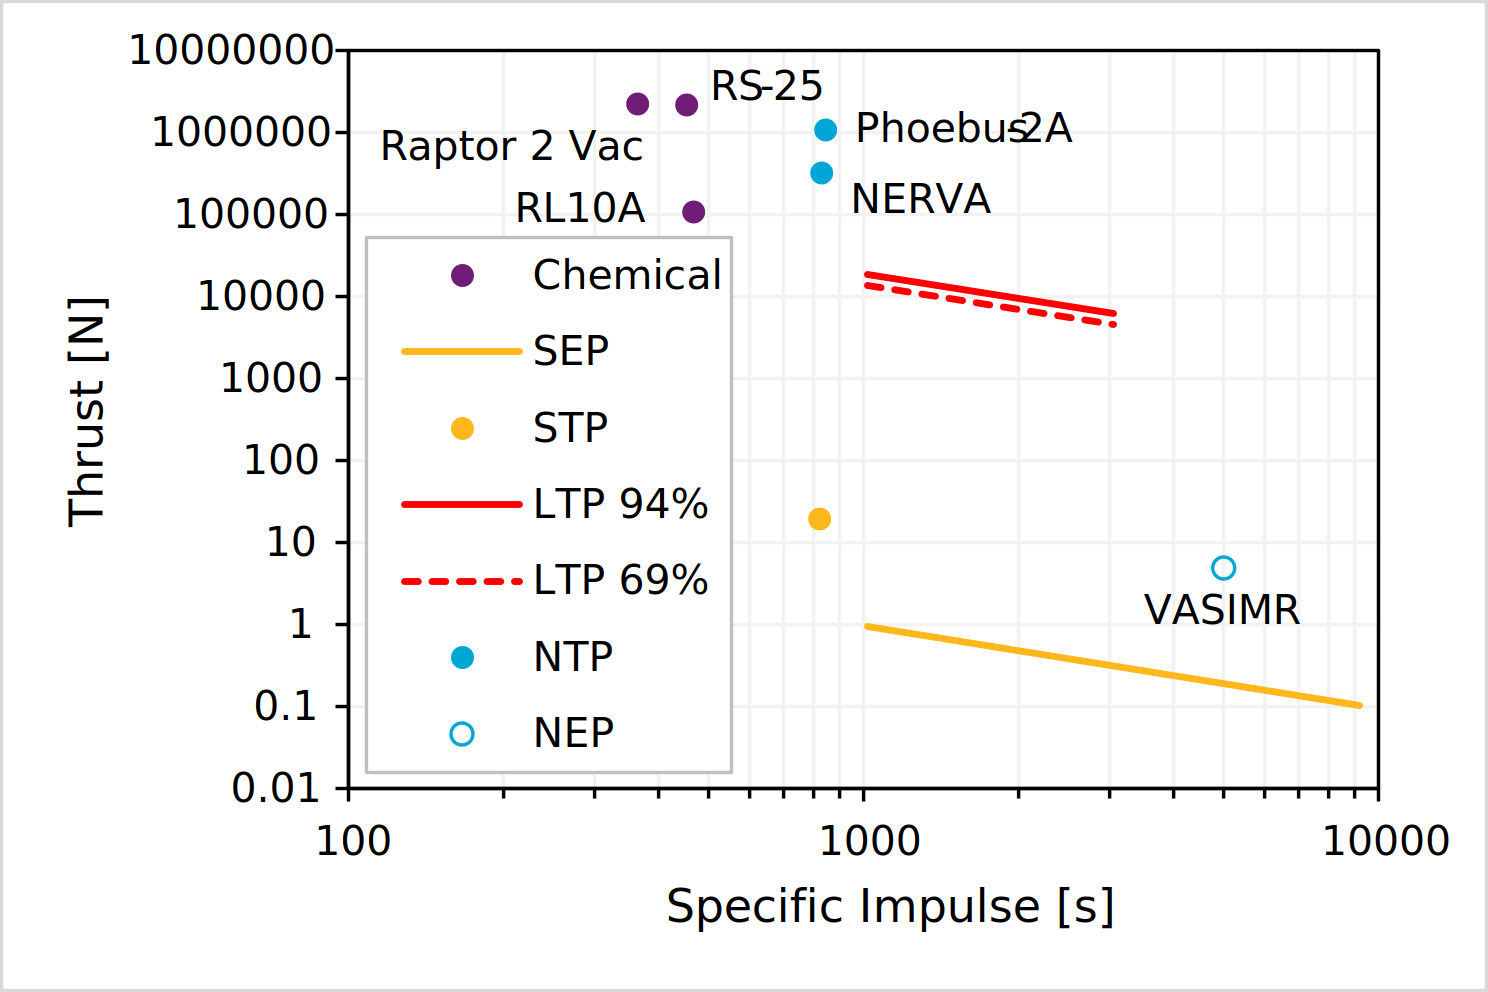
\includegraphics[width=0.9\textwidth]{assets/1 intro/propulsionComparison2.pdf}
            \caption[Comparison of various space propulsion systems]{Comparison of various space propulsion systems based on their specific impulse and thrust. References: Chemical~\cite{l3harrisRL10Engine2023,l3harrisRS25Engine2023,belluscioSpaceXAdvancesDrive2014}, Solar-Electric Propulsion (SEP)~\cite{aerojetrocketdyneNEXTCNASAEvolutionary2022}, Solar-Thermal Propulsion (STP)~\cite{woodcockEvaluationSolarThermal}, LTP~\cite{duplayDesignRapidTransit2022,shojiPerformanceHeatTransfer1976}, NTP~\cite{koenigExperienceGainedSpace1986}, Nuclear-Electric Propulsion (NEP)~\cite{adastraTechnology2013}}
            \label{fig:propulsion_comparison}
        \end{figure}

        The work done in this thesis supports the efforts of research performed at McGill University on LTP. \textcite{duplayDesignRapidTransit2022} considered the application of LTP for a 45-day transit to Mars, showing that this concept could plausibly deliver a 1-ton payload to the planet for less than 1~\% of the propellant required by an equivalent mission powered by a chemical rocket engine. This study attracted significant attention, motivating the group to pursue further modelling and experimental research efforts. This Master's thesis documents the design of a Laser-Sustained Plasma (LSP) facility for propulsion applications, and reports preliminary data on LSP absorption, behavior in co-axial flow conditions, and thrust characteristics of this LTP thruster laboratory model.
    \chapter{Background}
    To best understand the work done in this thesis, some background information on laser-thermal propulsion is provided in this chapter. This is an abridged version of the literature review~\cite{duplayReviewLaserThermalPropulsion2022} written before starting this thesis, which can be consulted for an in-depth study of past literature. The working principle of LTP will first be discussed, including a brief discussion of DEP and alternate concepts that also fall under the LTP category. A thorough discussion of LSP, the physics powering the laser-plasma LTP thruster, will then be given. Finally, an overview of the experimental work done on both LSP and LTP will be provided.

    This chapter will then end on stating research objectives for this thesis, derived from the findings of the literature review summarized here.

    \section{Working principle}
        LTP is a directed-energy propulsion concept, a class of propulsion systems where energy is beamed to a spacecraft, usually as a laser. This energy is then used for propulsion in some shape or form. This allows the spacecraft to forego much of its power and propulsion system mass, increasing its propellant or payload mass budget. Some applications of DEP, such as lightsails, even bypass the rocket equation altogether, making them a promising avenue for interstellar missions, as shown by \textcite{lubinRoadmapInterstellarFlight2022}. \citeauthor{lubinRoadmapInterstellarFlight2022} proposes modular, scalable fiber-laser arrays operating at \qty{1064}{nm} to beam the required MW to GW of power necessary to propel interplanetary and interstellar spacecraft. This specific laser wavelength transmits with virtually no losses through the atmosphere (\textcite{geminiobservatorySites2020}), and perturbations caused by atmospheric turbulence can be readily corrected using adaptive optics technology already in use in astronomy, as discussed by \textcite{eckelLaserPropulsionSystems, hettelBeamPropagationSimulation2021}.

        ``Laser-thermal propulsion'' itself encompasses several concepts where the laser is used to energize a propellant stored aboard the spacecraft. \textcite{kantrowitzRelevanceSpace1971} first proposed this idea as way to reduce launch costs. Such concepts include pulsed concepts that ablate solid propellant or cause laser-supported detonations, as studied by \textcite{myraboPowerBeamingTechnologyLaser1984}, or laser heat-exchanger systems, as proposed by \textcite{kareLaserpoweredHeatExchanger1995}. 
        
        The present work focuses on continuous-wave (CW) laser-plasma propulsion, proposed by \textcite{noredApplicationHighPower1976} and studied in detail by \textcite{keeferLaserSustainedPlasmas1989}: as illustrated in \autoref{fig:overview}, a continuous laser is used to sustain a laser-sustained plasma (LSP)\footnote{This physical phenomenon is also referred to as ``optical plasmotron'', ``light spark'', ``continuous optical discharge (COD)'', or ``laser-supported combustion (LSC) wave'' in the literature.} core within a thrust chamber (\autoref{fig:overview_chamber}). This plasma absorbs laser energy and redistributes it to the propellant gas via conduction and radiation. The heated propellant is then expelled through a high-area ratio nozzle, like any other vacuum-optimized thermal rocket engine. It should be highlighted that although the LSP can attain temperatures of \qtyrange{20000}{30000}{K} (\textcite{noredApplicationHighPower1976}), it is thought to be relatively small compared to the thrust chamber size. The heat from the LSP core is distributed to the cooler gas flowing past it, resulting in a bulk propellant temperature\footnote{``Average'' temperature---resulting temperature if the heat in the flow is distributed evenly} at the nozzle inlet of ``only'' 10~000~K (\textcite{duplayDesignRapidTransit2022}). As will be discussed further in \autoref{sec:background_lsp}, the LSP core's position and size is easily controlled by the laser beam geometry (\textcite{keeferLaserSustainedPlasmas1989}), requiring no additional confinement mechanisms (such as the ones seen in fusion propulsion concepts) to separate the plasma from the chamber walls. 
        
        \begin{figure}[t]
            \centering
            \begin{subfigure}[t]{0.64\textwidth}
                \centering
                \includegraphics[width=\textwidth]{assets/2 background/overview_ltp.pdf}
                \caption{Spacecraft}
                \label{fig:overview_spacecraft}
            \end{subfigure}
            \begin{subfigure}[t]{0.64\textwidth}
                \centering
                \includegraphics[width=\textwidth]{assets/2 background/chamber.pdf}
                \caption{Thrust chamber}
                \label{fig:overview_chamber}
            \end{subfigure}
            \caption[Overview of a CW laser-plasma LTP system]{Overview of a CW laser-plasma LTP system, adapted from \textcite{duplayDesignRapidTransit2022}}
            \label{fig:overview}
        \end{figure}

        As alluded to in the \nameref{chp:intro}, the key advantage of laser-thermal propulsion over chemical propulsion is its ability to deliver far greater exhaust velocities. Following from thermal rocket theory (\textcite{zandbergenAE4S01ThermalRocket2020}), the limiting exhaust velocity $v_\text{ex, max}$ of a thermal rocket motor depends on \autoref{eq:isp}, where $\gamma$ is the specific heat ratio of the propellant gas, $R_\text{u}$ is the universal gas constant, $\mathcal{M}$ is the propellant molar mass, and $T_\text{c}$ is the chamber temperature.
        \begin{equation}
            I_\text{sp, max}g_0 = v_\text{ex, max} \propto \sqrt{2\frac{\gamma}{\gamma-1}\frac{R_\text{u}}{\mathcal{M}}T_\text{c}} \label{eq:isp}
        \end{equation}
        All other parameters being equal, a thermal rocket engine operating at a higher chamber temperature will thus have a greater limiting exhaust velocity. By decoupling the thermal input from the propellant choice, unlike chemical thrusters whose chamber temperature is limited by their chemical reaction's adiabatic temperature, a laser-thermal rocket engine can readily attain temperatures of up to 10~000~K at the nozzle inlet, resulting in a specific impulse of more than 1000~s, as shown by \textcite{noredApplicationHighPower1976} in \autoref{fig:nored_Isp}.

        \begin{figure}[h]
            \centering
            \includegraphics[width=0.7\textwidth]{assets/2 background/nored_ltpIsp.png}
            \caption[Theoretical specific impulse attained for a given hydrogen temperature]{Theoretical specific impulse attained for a given hydrogen temperature at the nozzle inlet, by \textcite{noredApplicationHighPower1976}. The specific impulse is bounded by two cases: 1.~the exhaust products maintain chemical equilibrium as they cool and expand through the nozzle; 2.~the composition of the exhaust is ``frozen''}
            \label{fig:nored_Isp}
        \end{figure}

        Some practical issues with this concept do remain. Although it is well understood that the high propellant temperatures that could be achieved by LTP would result in \qtyrange{1000}{3000}{s} of specific impulse (with hydrogen), whether or not the heat deposited in the LSP can be transferred to all the propellant flow with minimal losses is a critical issue. This problem was studied in-depth by \textcite{shojiPerformanceHeatTransfer1976}, who performed a thorough analysis of heat transfer within two LTP engines, proposing seeding the flow with carbon particles as a solution to reduce radiative heat losses to the chamber walls. Their analysis showed that such losses could be reduced to 4.5~\% of the input laser power, for hydrogen seeded with 50~\% carbon (by weight). While this is promising, such a system has yet to be tested experimentally. Furthermore, as suggested by \autoref{eq:isp}, the introduction of higher molar-mass carbon particles is associated with a penalty in the resulting specific impulse: \citeauthor{shojiPerformanceHeatTransfer1976}'s models show a decrease in theoretical specific impulse of around 25~\%.

        Cooling is also an issue. Even with the inclusion of carbon seeding, the magnitude of laser power considered for DEP (MW to GW) makes 4.5~\% of input power radiated to the thruster walls considerable. The propellant temperatures associated with high specific impulse are also far greater than the ones typically encountered by conventional thermal rocket engines, potentially necessitating new cooling strategies (\textcite{noredApplicationHighPower1976}). Thankfully, many of these cooling issues are similar in nature and magnitude to those encountered in Gas-Core Nuclear Rockets (GCNR), a sub-type of NTP. \textcite{kascakNozzleCavityWall1971} discusses a hydrogen GCNR operating at temperatures and specific impulses of the same order of magnitude, suggesting that a combination of transpiration cooling and gas seeding would be sufficient.

    \section{Laser-Sustained Plasma} \label{sec:background_lsp}
        One might wonder why bother with plasma at all. If the laser radiation could be deposited evenly in the propellant flow, little to no mixing would be needed and peak temperatures would be lower. Unfortunately, the use of lasers to directly heat hydrogen propellant has a major flaw: hydrogen gas does not absorb 1-\unit{\um}-wavelength radiation at room temperatures. Hydrogen only begins to absorb this wavelength at around 10~000~K, as shown by \textcite{glumbConceptsStatusLasersupported1984}: ``The paradox is that hydrogen cannot absorb any laser radiation unless it is already hot.'' They were considering 10.6 \unit{\um} laser radiation, but this also holds for 1.06 \unit{\um}. The reason for this being that this wavelength does not match hydrogen's resonance absorption bands, whereby radiation is absorbed in the rotational or vibrational modes of a molecule. The main absorption mechanism in LSP is \emph{inverse brehmsstrahlung} (IB): free electrons absorb radiation across a continuous spectrum (as opposed to specific wavelengths) during collisions with ions in the plasma (\textcite{keeferLaserSustainedPlasmas1989}). \textcite{johnstonCorrectValuesHighfrequency1973} showed that the radiation absorption coefficient $\alpha$ [1/m] can be calculated with \autoref{eq:ib_absorption}, where $Z$ is the ionic charge, $n_\mathrm{e}$ is the electron density, $\nu$ is the radiation frequency, $k_\mathrm{B}$ is the Boltzmann constant, and $T_\mathrm{e}$ is the electron temperature [K]. $\ln{\Lambda}$, the Coulomb logarithm, and $\nu_\mathrm{p}$, the plasma frequency, will be discussed in further detail in \autoref{chp:models}.
        \begin{equation}
            \alpha = \frac{7.8\times 10^{-7}Zn_\mathrm{e}^2\ln{\Lambda}}{\nu^2(k_\mathrm{B}T_\mathrm{e})^{3/2}} \left(1-\frac{\nu_\mathrm{p}^2}{\nu^2}\right)^{-1/2} \label{eq:ib_absorption}
        \end{equation}

    \section{Past experiments}
    \chapter{Facility design}
    Since there was no existing LSP facility at McGill University, a considerable portion of this project revolved around the design and fabrication of an LSP generator. This chapter will discuss the major design requirements of such a system, the selection of appropriate solutions, and the assembly, integration, and testing process. Several practical issues were encountered in developing the LSP generator, which are rarely mentioned in the experimental LSP literature. They will be documented in detail in this report in the hopes that this can facilitate future work in this field.

    \section{Needs and requirements}


        \begin{statement}{Need statement} 
            In order to properly define the problem solved by a system, a need statement is needed.
        \end{statement}

        \subsection{Existing hardware}
            The laser made available for this project was the most important driver of many design decisions. Wether they are for interstellar-class lightsails as envisioned by \textcite{lubinRoadmapInterstellarFlight2022}, or interplanetary missions powered by electric propulsion as proposed by \textcite{sheerinFastSolarSystem2021}, fiber lasers operating at the 1064-nm-wavelength are currently favored for many DEP applications. Since LTP is proposed as an additional DEP concept within this ecosystem, this experimental work aimed to match this laser wavelength.

            An IPG Photonics YLR-300/3000-QCW-MM-AC Ytterbium fiber laser (seen in \autoref{fig:laser_laser}) was generously loaned to the IFERG by the Royal Military College of Canada. This is an infrared laser primarily designed for welding, drilling, and cutting. It is capable of operating in both pulsed and continuous modes at a wavelength of \qty{1070}{nm}. Its key specifications are summarized in \autoref{tab:laser_spec}. A complete calibration report for the laser can be found in \autoref{chp:app_YLR}. An IPG Photonics P30-001736 collimator head (seen in \autoref{fig:laser_collimator}) was also acquired for the laser, forming a 13.6-mm-diameter beam at its output. The collimator's calibration report can be found in \autoref{chp:app_Collimator}.

            Although a practical LTP system would likely operate in continuous mode, the YLR laser's pulsed mode was of particular interest in this project. As discussed in \autoref{sec:background_lsp}, laser power is a critical factor in the ability to achieve a steady LSP. The YLR laser is not only capable of pulsing at an order of magnitude above its CW power rating, but it is able to do so for several milliseconds, a relatively long-pulse in the world of laser physics. This pulse is in fact so long that it is considered to be in the CW regime as far as laser damage is concerned (\textcite{thorlabsNBK7PlanoConvexLenses}), hence the \emph{Quasi}-Continuous-Wave (QCW) designation of this laser. This capability enables running very high power experiments without investing in far more expensive (and dangerous) CW kW-class lasers, though the 10~ms timescale imposes a major constraint on the facility design and experimental methodology.
        
            \begin{table}
                \centering
                \caption{Summary of nominal laser specifications}
                \label{tab:laser_spec}
                \begin{tabular}{@{}lrl@{}}
                    \toprule
                    \textbf{Parameter}            & \textbf{Quantity} & \textbf{Unit} \\ \midrule
                    Wavelength                    & 1070              & nm            \\
                    Maximum CW Power              & 300               & W             \\
                    Maximum Pulse Power           & 3000              & W             \\
                    Maximum Pulse Duration (3 kW) & 10                & ms            \\
                    Maximum Pulse Energy          & 30              & J             \\ \bottomrule
                    \end{tabular}
            \end{table}

            \begin{figure}[h]
                \centering
                \begin{subfigure}[t]{0.6\textwidth}
                    \centering
                    \includegraphics[height=2.6in]{assets/3 design/laser.jpg}
                    \caption{IPG Photonics YLR-300/3000-QCW-MM-AC Laser}
                    \label{fig:laser_laser}
                \end{subfigure}
                \begin{subfigure}[t]{0.35\textwidth}
                    \centering
                    \includegraphics[height=2.6in]{assets/3 design/collimator_r.jpg}
                    \caption{Laser collimator head}
                    \label{fig:laser_collimator}
                \end{subfigure}
                \caption{Laser system used for this project}
                \label{fig:laser}
            \end{figure}

        \subsection{Requirements}

            \begin{table}[h]
                \renewcommand{\arraystretch}{1.3}
                \centering
                \caption{Top-level design requirements for the LTP laboratory model (the ``thruster'')}
                \label{tab:lttmReq}
                \begin{tabular}{l>{\raggedright}p{0.4\textwidth}p{0.4\textwidth}<{\raggedright}}
                    \toprule
                    \textbf{Identifier}  & \textbf{Requirement}   & \textbf{Rationale} \\
                    \midrule
                    LTTLM-1     & The thruster shall operate at a maximum laser power of \qty{3}{kW} at a wavelength of \qty{1070}{nm}    & This is the laser system made available for this experiment \\
                    LTTLM-2     & The thruster shall operate using gaseous argon at room temperature as a propellant & The past experiments used for comparison also used argon \\
                    LTTLM-3     & The thruster shall operate at a maximum design pressure of 2~\unit{MPa} & This should allow the generation of LSP even in continuous-wave laser modes \\
                    LTTLM-4     & The thruster shall allow visible observation of the LSP in the thrust chamber & This enables high-speed imaging of the plasma and the remote measurement of its temperature \\
                    LTTLM-5     & The thruster shall provide chamber pressure and gas temperature data   & This permits the estimation of stagnation conditions for the heated propellant \\
                    LTTLM-6     & The thruster shall allow the measurement of absorbed laser power   & This is one of the major energy losses to be determined \\
                    \bottomrule
                \end{tabular}
            \end{table}

    \section{Design process}
        \subsection{Test section}
            The requirements for the Laser-Thermal Thruster Laboratory Model (LTTLM) are listed in \autoref{tab:lttmReq}. In summary, the thruster model should be a pressurized vessel featuring one or more windows to allow laser input and optical viewing of the LSP. Furthermore, this vessel should allow the integration of various instrumentation systems. The design and manufacture of such a vessel would have required a significant amount of time, so the alternative of re-purposing hardware from a different project was considered first. This hardware's specifications could be compared to the requirements, and modifications could be made if necessary.

            Coincidentally, \textcite{kokkalisOnsetCavitationDynamically2023} at the neighboring McGill Fluid Dynamics Lab was undertaking research into cavitation effects within piston-cylinder assemblies. Their apparatus included cylindrical sections designed to withstand high dynamic pressures encountered in their experiments, and featured windows or transparent walls to track the onset of cavitation with high-speed cameras. The design was modular, allowing the installation of various endcaps with different functions. This theoretically fulfilled requirements LTTLM\nobreakdash-2 to LTTLM\nobreakdash-4. One particular test section (pictured in \autoref{fig:cavitation}, detailed drawings can be found in \autoref{chp:app_CavitatorDrawings}) had been fabricated with a set of instrumentation ports and polycarbonate windows spanning the length of the cylinder. This test section had been tested in a few experiments but was found to be inadequate, as gaps around the ports and windows were sources of parasitic cavitation.

            \begin{figure}[h]
                \centering
                \begin{subfigure}[t]{0.46\textwidth}
                    \centering
                    \includegraphics[width=\textwidth]{assets/3 design/cavitatorDrawing.pdf}
                    \caption{Assembly schematic}
                    \label{fig:cavitation_schematic}
                \end{subfigure}
                \begin{subfigure}[t]{0.49\textwidth}
                    \centering
                    \includegraphics[width=\textwidth]{assets/3 design/cavitationSection.jpg}
                    \caption{Photograph of the test section fitted with a gas feed line}
                    \label{fig:cavitation_photo}
                \end{subfigure}
                \caption{Cavitation test section}
                \label{fig:cavitation}
            \end{figure}

            As seen in \autoref{tab:lttmReq_partialVerif}, this apparatus was verified against the requirements set in \autoref{tab:lttmReq} to determine what retro-fitting activities would be needed to use it as an LTP thruster model. It was found that very little retrofitting work was required in order to use it as an LSP generator: special instrument plugs could be created, and special laser window endcaps were needed to seal the apparatus while allowing the laser to enter the test section. To operate the system as a thruster, a separate nozzle endcap could be made. Finally, as spectrometry was planned to be used for plasma temperature determination, the polycarbonate side windows would have to be exchanged for UV-grade quartz windows, which would allow a broader spectrum of radiation to pass through.
            
            However, using this test section would not come without a set of drawbacks. Its original intent made it unoptimized to work as a laser-thermal thruster model for the following reasons:
            \begin{enumerate}
                \item Though its thick stainless steel construction made it very safe for the operating pressures of the project, it also made it heavy. The superfluous mass would make frictional loads on a thrust bench far more significant than for a custom-designed, lightweight thruster model.
                \item Its length forces the use of long focal-length lenses to focus the laser into the test section. Such long lenses would create a high {\itshape f}-number beam, which could affect how easily a stable LSP could be achieved, as discussed in \autoref{sec:background_lsp}. While shorter lenses would still be able to focus the laser into the chamber, the beam past the focal point would diverge quickly and hit the test section walls, affecting laser absorption measurements at best, or damaging experimental apparatus at worst.
                \item Instrumentation ports are available only on one side of the cylinder. The lack of opposing ports constrains the design of certain ignition methods, such as spark igniters.
            \end{enumerate}



            \begin{table}[h]
                \renewcommand{\arraystretch}{1.3}
                \centering
                \caption{Verification of LTTLM requirements for the cavitation apparatus}
                \label{tab:lttmReq_partialVerif}
                \begin{tabular}{l>{\raggedright}p{0.53\textwidth}p{0.27\textwidth}<{\raggedright}}
                    \toprule
                    \textbf{Identifier} & \textbf{Requirement}                                                                   & \textbf{Status}                   \\ \midrule
                    LTTLM-1             & The thruster shall operate at a maximum laser power of \qty{3}{kW} at a wavelength of \qty{1070}{nm} & Requires laser windows            \\
                    LTTLM-2             & The thruster shall operate using gaseous argon at room temperature as a propellant     & Fulfilled                         \\
                    LTTLM-3             & The thruster shall operate at a maximum design pressure of 2 MPa                       & Fulfilled                         \\
                    LTTLM-4             & The thruster shall allow visible observation of the LSP in the thrust chamber          & Fulfilled                         \\
                    LTTLM-5             & The thruster shall provide chamber pressure and gas temperature data                   & Requires special instrument plugs \\
                    LTTLM-6             & The thruster shall allow the measurement of absorbed laser power                       & Requires laser windows            \\ \bottomrule
                \end{tabular}
            \end{table}

    \section{Integration and test}
    \chapter{Modelling} \label{chp:models}
    
    \chapter{Experiments}
    The results of the first experiments performed on the LSP facility are presented here. These include an exploration of ignition methods and their reliability, the attempted replication of power-threshold experiments seen in LSP literature, and the analysis of LSP's absorption, heat deposition, and spectral characteristics. Preliminary flowing data is also presented and contrasted with the static case.

    \autoref{fig:finalsetup_static} provides an overview of the instrumentation used in static experiments and their relative positions.

    \begin{figure}[h]
        \centering
        \includegraphics[width=0.85\textwidth]{assets/5 results/finalsetup_static}
        \caption{Static configuration of the test section}
        \label{fig:finalsetup_static}
    \end{figure}

    \section{Preliminary ignition experiments} \label{sec:ignitiontest}
        Once the necessary components of the experiment were integrated, a preliminary testing campaign began to attempt to ignite LSP. The hope was to resolve any unforeseen practical issues, then quickly move on to replicating the power threshold experiments of past LSP literature~\cite{zimakovInteractionNearIRLaser2016,matsuiGeneratingConditionsArgon2019,luCharacteristicDiagnosticsLaserStabilized2022}. The test campaign aimed to answer two questions:
        \begin{itemize}
            \item Can LSP be achieved with this experimental setup?
            \item How reliable is LSP ignition with this system?
        \end{itemize}
        To answer these questions, experimental trials would be run in conditions most favorable to steady LSP formation, i.e. at maximum laser power and maximum test section pressure: \qty{3}{kW} and \qty{20}{bar}. Successful ignition would be determined based on two independent measures:
        \begin{enumerate}
            \item The high-speed camera should be able to image the LSP growing and propagating towards the laser source over the course of the laser pulse, as consistently documented in LSP literature.
            \item A measurable drop in laser energy reaching the Gentec power meter should be observed.
        \end{enumerate}
        LSP would only be deemed to have successfully ignited if the expected behavior was observed with both instruments.

        \subsection{Spark-ignition}
            Laser alignment was immediately found to be a non-trivial problem. In order to successfully ignite the LSP, the laser must be focused onto the arc generated by the spark igniter. To maximize the chance of ignition, the laser flux at the arc must be as great as possible, so the focused laser dot must be as small as possible. This makes alignment tolerances much stricter, as the laser is less likely to be incident on the thin arc at all.

            Compounding this issue was the fact that the path taken by the arc between both electrode tips was not consistent. As seen in \autoref{fig:sparkAlignment}, the location of the arc was highly variable: although an average arc path could be determined, the arc could form up to \qty{1}{mm} away. This made it impossible to ensure consistent alignment between the arc and the laser focus. This issue could be alleviated by repeatedly triggering the spark, but the smart coil had a nominal delay of \qty{3}{ms} between sparks, only allowing up to three ignition attempts within a single laser pulse, making this approach of little viability for high-power pulse laser tests. Repeated sparks could be used with CW laser operation at \qty{300}{W}, but the lower laser power also reduces the likelihood of successful LSP ignition.

            \begin{figure}[h]
                \centering
                \begin{subfigure}[t]{0.47\textwidth}
                    \centering
                    \includegraphics[]{assets/3 design/sparkAlignment_one.jpg}
                    \caption{Single arc generated by the spark igniter}
                    \label{fig:sparkAlignment_one}
                \end{subfigure}
                \hfill
                \begin{subfigure}[t]{0.47\textwidth}
                    \centering
                    \includegraphics[]{assets/3 design/sparkAlignment.jpg}
                    \caption{Several arcs stacked together to create a ``heatmap'' of arc formation. Note the large variance in the path taken by the arc.}
                    \label{fig:sparkAlignment_heatmap}
                \end{subfigure}
                \caption[Composite photos made during a typical spark-laser alignment procedure]{Composite photos made during a typical spark-laser alignment procedure. The gray-scale background, blue arcs, and red guide laser photos were taken separately then stacked together to be able to compare the relative position of the arcs and laser.}
                \label{fig:sparkAlignment}
            \end{figure}

            In addition, the laser could not be aligned without placing reflecting or scattering material in the beam path. As seen in \autoref{fig:sparkAlignment}, a target must be placed near the ignition point to perform the alignment (and also serves as a scale indicator). However, this alignment target had to be removed to pressurize the test section, which was required both to determine the spark location, and to perform the LSP ignition test. Pressurization cycles and the placing/removal of this target made the alignment process slow and cumbersome. Alignment with the arcs could not be confirmed visually since the target could not be present when pressurizing the test section.

            Despite these difficulties, several attempts were made to ignite LSP with this method, and a few were successful. The first successful test was performed at \qty{10.0}{bar} with a full power pulse (\qty{30.8}{J}). A paper target had been placed next to the electrodes to facilitate alignment, so no measurements were made of the pulse energy transmitted through the plasma for the first few successful tests. However, high-speed footage showed strong evidence of plasma formation: a bright flash saturating the camera sensor, igniting at the time of spark formation, as seen in \autoref{fig:lsp1}. Such a flash had never been observed in past (failed) ignition tests. Although this suggested that some plasma had been formed, there was a possibility that the alignment target was affecting the experiment and may even have contributed to the ignition. The footage showed evidence of particles being ejected from the area around the ignition point, possibly due to the interaction between the laser, plasma, and the paper target.

            \begin{figure}[h]
                \centering
                \begin{subfigure}[t]{0.32\textwidth}
                    \centering
                    \includegraphics[width=\textwidth]{assets/3 design/LSP1_frames/20.jpg}
                    \caption{2.0~ms}
                    \label{fig:lsp1_20}
                \end{subfigure}
                \hfill
                \begin{subfigure}[t]{0.32\textwidth}
                    \centering
                    \includegraphics[width=\textwidth]{assets/3 design/LSP1_frames/30.jpg}
                    \caption{3.0~ms}
                    \label{fig:lsp1_30}
                \end{subfigure}
                \hfill
                \begin{subfigure}[t]{0.32\textwidth}
                    \centering
                    \includegraphics[width=\textwidth]{assets/3 design/LSP1_frames/75.jpg}
                    \caption{7.5~ms}
                    \label{fig:lsp1_75}
                \end{subfigure}
                \caption{High-speed footage frames of first successful LSP ignition}
                \label{fig:lsp1}
            \end{figure}

            The experiment was repeated with the target several times, ensuring that the flash was not the result of merely burning a hole through the paper target. In addition, the exposure settings were adjusted (increasing the ND filter to ND2048 and setting the aperture to \textit{f}/22) to provide a clearer view of the brightest part of the frame, the LSP core. A snapshot of the resulting footage is shown in \autoref{fig:lsp3}, revealing a slender plasma core, approximately contained within the focused laser beam (note the thinner right tip of the LSP compared to the left tip). The plasma was observed to grow towards the source of the laser, as reported in the experimental LSP literature. This appearance and growth behavior provided additional evidence that these tests were truly achieving laser-sustained plasma, as opposed to some other phenomenon.

            \begin{figure}[h]
                \centering
                \includegraphics[]{assets/3 design/LSP3_annotated.jpg}
                \caption[Third successful LSP test ignited by arc discharge]{Third successful LSP test ignited by arc discharge. Snapshot from just before the end of the laser pulse. Dimension is approximate.}
                \label{fig:lsp3}
            \end{figure}

            To provide complete confidence that this indeed was LSP, more experiments were performed without the paper target. This allowed the measurement of the laser energy that was not absorbed by the plasma and would confirm that the LSP is ignited purely by the spark, as opposed to ablated material from the paper target. With a fully uninterrupted beam path, the power meter reported a 70 to 80\% drop in laser pulse energy during a test, suggesting that significant laser absorption was occurring in the plasma. This thus satisfied the second criterion for determining successful LSP ignition.

        \subsection{Wire-ignition}
            As power-threshold experiments were underway, as discussed in \autoref{sec:results_powerthreshold}, it became apparent that the reliability of spark-ignition was unsatisfactory. The inability to consistently arc through the laser beam meant that most ignition attempts would fail, especially below full laser power. Reliability of the spark ignition system was estimated between 10\% and 50\% depending on conditions.

            Private communications with Todd and Nassar (involved in \cite{akarapuNumericalModelLasersustained2009,nassarInvestigationLasersustainedPlasma2012}) highlighted the difficulty of spark ignition, and motivated the change to a solid-target system, with the use of thin metallic wire as an ignition target. Tungsten had been used successfully in past LSP experiments, such as those of \textcite{toyodaThrustPerformanceCW2002}, so \qty{0.254}{mm} (0.01") Tungsten wire was acquired and placed in the beam path as a target.

            Wire-ignition proved to be easier to work with, as laser alignment was simpler. However, it did not guarantee ignition either---wire ignition's greater reliability revealed other important factors in consistently achieving LSP:
            \begin{itemize}
                \item Axial positioning of the laser focus such that it coincides with the target is crucial to generate the ``seed'' cloud of electrons necessary for LSP ignition.
                \item Ensuring high Argon purity in the chamber was also found to be important. Venting of residual air in the system done by performing several pressurization-vent cycles with Argon---at least 3 cycles up to \qty{5}{bar}---before final pressurization to the test pressure. While this was sufficient for tests at \qty{10}{bar} and above, additional cycles were found to improve ignition reliability at low pressures (\qtyrange{3}{10}{bar}).
            \end{itemize}
            Factors that were hypothesized to impact reliability but ultimately were found to have little to no impact include:
            \begin{itemize}
                \item Focusing the laser on the same spot on a wire across several tests
                \item Touching/dirtying the wire before installing it in the test section
                \item Sanding/cleaning the wire before installing it in the test section
            \end{itemize}
            Once these reliability factors were identified and controlled, wire ignition proved to be highly reliable, attaining practically 100\% reliability.

        \subsection{Early LSP observations}
            These early ignition tests already allowed the observation of LSP. \autoref{fig:ignition_frames} depicts the initial growth of LSP ignited off a Tungsten wire, showing rapid growth over a fraction of a millisecond. Under the right ignition conditions, plasma would form practically as soon as the laser was turned on, before the Tungsten wire had time to heat up and melt off. This quick ignition would prove to be a useful property when combined with stepped-pulse profiles in later power threshold experiments.

            \begin{figure}[h]
    \centering
    \begin{subfigure}[t]{0.3\textwidth}
        \centering
        \includegraphics[width=\textwidth]{assets/5 results/ignitionFrames/16.jpg}
        \caption{\qty{1.6}{ms}}
        \label{fig:ignition_frames_16}
    \end{subfigure}
    \hfill
    \begin{subfigure}[t]{0.3\textwidth}
        \centering
        \includegraphics[width=\textwidth]{assets/5 results/ignitionFrames/17.jpg}
        \caption{\qty{1.7}{ms}}
        \label{fig:ignition_frames_17}
    \end{subfigure}
    \hfill
    \begin{subfigure}[t]{0.3\textwidth}
        \centering
        \includegraphics[width=\textwidth]{assets/5 results/ignitionFrames/18.jpg}
        \caption{\qty{1.8}{ms}}
        \label{fig:ignition_frames_18}
    \end{subfigure}
    \begin{subfigure}[t]{0.3\textwidth}
        \centering
        \includegraphics[width=\textwidth]{assets/5 results/ignitionFrames/19.jpg}
        \caption{\qty{1.9}{ms}}
        \label{fig:ignition_frames_19}
    \end{subfigure}
    \hfill
    \begin{subfigure}[t]{0.3\textwidth}
        \centering
        \includegraphics[width=\textwidth]{assets/5 results/ignitionFrames/20.jpg}
        \caption{\qty{2.0}{ms}}
        \label{fig:ignition_frames_20}
    \end{subfigure}
    \hfill
    \begin{subfigure}[t]{0.3\textwidth}
        \centering
        \includegraphics[width=\textwidth]{assets/5 results/ignitionFrames/21.jpg}
        \caption{\qty{2.1}{ms}}
        \label{fig:ignition_frames_21}
    \end{subfigure}
    \caption[LSP ignition via tungsten wire]{LSP ignition via tungsten wire: \qty{3080}{W}, \qty{20.29}{bar}. The white line at the bottom of each frame is \qty{10}{mm} long. \shotsettings{LSP1\_PS1}{0.1}{22}{2048}}
    \label{fig:ignition_frames}
\end{figure}

            Selected frames of an entire LSP lifetime are shown in \autoref{fig:growth_frames}. The initially rapid LSP growth ($\sim$\qty{9}{m.s^{-1}}) slows down as it approaches steady conditions, with the front speed decreasing to less than \qty{1}{m.s^{-1}} by the end of the laser pulse. Steady-state conditions have thus not been truly achieved with full-power, \qty{10}{ms} pulses. The LSP responded practically instantaneously to the end of the laser pulse, as it dissipated from the high speed footage in the span of 1--2 frames.
            
            \input{assets/5 results/1msFrames/1msFrames.tex}
    \clearpage
    \section{Power threshold} \label{sec:results_powerthreshold}
        Once LSP ignition had been confirmed, work began on reproducing power threshold experiments, a frequent topic in LSP research. The aim of this experiment is to determine the minimum laser power required to sustain a steady plasma, at a given pressure. Knowing this power threshold is useful to establish the operation bounds of an LSP facility, whether it is a laboratory experiment or a laser-thermal thruster. Several of such experiments have been performed for Argon with fiber-lasers: the work of \textcite{zimakovInteractionNearIRLaser2016, matsuiGeneratingConditionsArgon2019,luCharacteristicDiagnosticsLaserStabilized2022} will thus be used for comparison.
        
        \subsection{Methodology}
            The test section would be pressurized with Argon to a desired pressure between 3 and 20~bar. Then, determining the power threshold was done through a process akin to a binary search or bisection root-finding algorithm in computer science: LSP would be ignited first at the maximum setpoint power to confirm that the laser and igniter were aligned such that LSP was achievable. Power would then be reduced to a point far below the threshold (10\% power) to confirm that LSP was not achieved. This brackets the threshold point. Subsequent tests would be performed at a power setpoint in the middle of this iteratively shrinking bracket, until the threshold was determined to be within approximately \qty{50}{W} below the last successful LSP test.

            This series of tests were performed with both spark and wire ignition. One issue encountered with wire ignition was that while lower laser powers could theoretically sustain LSP, they would not necessarily be sufficient to ignite it. To circumvent this issue, stepped laser pulse profiles were used instead of constant laser power. An example of such a pulse is shown in \autoref{fig:pulse_stepProfile}: the pulse begins at 100\% setpoint power for \qty{0.5}{ms} to initiate the LSP off of the Tungsten wire. The power would then be stepped down to the desired power level, which would be maintained for as long as possible to ensure that the LSP could re-adjust to steady conditions.

            \begin{figure}[h]
                \centering
                \includegraphics[]{assets/5 results/pulse_profile}
                \caption[Typical stepped-pulse profile: \texttt{05L33\_15}]{Typical stepped-pulse profile: \texttt{05L33\_15}. A complete list of stepped-pulse specifications can be found in \autoref{chp:app_pulseShapes}.}
                \label{fig:pulse_stepProfile}
            \end{figure}

            Whether LSP could be considered steady for a given test was determined by observing its behavior in the high-speed footage. It needed to fulfill two conditions:
            \begin{enumerate}
                \item The LSP is still visible at the end of the laser pulse
                \item The LSP is not visibly changing by the time the laser pulse ended, i.e., it is not shrinking or dimming significantly.
            \end{enumerate}
            As plasma brightness changed with laser power, the variable ND filter would be adjusted to determine whether a vanishing plasma was unstable or simply too dim to be picked up through the lens filters.

        \subsection{Results}
            The resulting power threshold plot can be seen in \autoref{fig:powerthreshold}. Both spark and wire ignition experiments are shown, along with data reported by \textcite{zimakovInteractionNearIRLaser2016,matsuiGeneratingConditionsArgon2019,luCharacteristicDiagnosticsLaserStabilized2022}. The use of wire ignition shows a significant improvement in the minimum power required to sustain LSP over the spark ignition method. The improved reliability and ease of alignment afforded by wire ignition enabled sustaining LSP down to hundreds of Watts, whereas spark ignition struggled to ignite and sustain LSP below \qty{1}{kW}. Note that the uncertainties indicated on the wire ignition data reflect the possible range in which the true power threshold lies and is not related to an uncertainty in the power measurement. \textcite{zimakovInteractionNearIRLaser2016} presented a model based on balancing input power with heat conduction ($P_\mathrm{h}$) and radiative losses ($P_\mathrm{r}$), to evaluate the power threshold as a function of pressure $P_\mathrm{t}$. This expression is reproduced here as \autoref{eq:zimakov_threshold}:
            \begin{equation} \label{eq:zimakov_threshold}
                P_\mathrm{t} = P_\mathrm{h} + P_\mathrm{r}
            \end{equation}
            \citeauthor{zimakovInteractionNearIRLaser2016}'s experiments had experimentally estimated the parameters of this equation for Argon as $p^2P_\mathrm{h} =$~\qty{26}{bar^2.kW} and $P_\mathrm{r} =$~\qty{240}{W}. This same model was fitted to this study's wire-ignited LSP data, yielding the following power threshold parameters: $p^2P_\mathrm{h} =$~\qty{11}{bar^2.kW} and $P_\mathrm{r} =$~\qty{178}{W}. These values can be interpreted, respectively, as the minimum laser power to sustain LSP at \qty{1}{bar}, and the limiting laser power under which no LSP can be sustained even at high pressures.

            The discrepancy in the power thresholds achieved across different experiments is due in part to the optical quality of the focused beam, as suggested by \textcite{luCharacteristicDiagnosticsLaserStabilized2022}, who have so far achieved the lowest power-threshold results for fiber-laser-sustained Argon plasma. As the literature data is all from spark-ignited experiments, direct comparisons to wire ignition tests may be limited. However, this suggests that a low power threshold can be readily achieved by a basic optical train and a simple wire-ignition system combined with stepped pulse profiles, competing with methodologies that require far greater precision and optical quality.

            Qualitative observations were made on the LSP's response to the step-down in laser power. As seen in \autoref{fig:lsp_stepdown}, the decrease in input power is immediately apparent, with the plasma shrinking and dimming as soon as the power is dropped. The LSP re-adjusts to new power conditions in less than a millisecond. In this particular case, the LSP remained stable until the end of the laser pulse, \qty{14.8}{ms} after the step-down in power.


            \begin{figure}[h]
                \centering
                \includegraphics[]{assets/5 results/powerthreshold}
                \caption[Pressure-Power LSP threshold exploration]{Pressure-Power LSP threshold exploration. \textcite{zimakovInteractionNearIRLaser2016}'s model is fitted to wire ignition data as the blue dashed line.}
                \label{fig:powerthreshold}
            \end{figure}

            \begin{figure}[h]
                \centering
                \begin{subfigure}[t]{0.32\textwidth}
                    \centering
                    \includegraphics[trim=7.6in 5.3in 2.4in 5.5in, clip, width=\textwidth]{assets/5 results/LSP34_PS28/20.jpg}
                    \caption{\qty{2.0}{ms}, before step-down}
                    \label{fig:lsp_stepdown_20}
                \end{subfigure}
                \hfill
                \begin{subfigure}[t]{0.32\textwidth}
                    \centering
                    \includegraphics[trim=7.6in 5.3in 2.4in 5.5in, clip, width=\textwidth]{assets/5 results/LSP34_PS28/21.jpg}
                    \caption{\qty{2.1}{ms}, after step-down}
                    \label{fig:lsp_stepdown_21}
                \end{subfigure}
                \hfill
                \begin{subfigure}[t]{0.32\textwidth}
                    \centering
                    \includegraphics[trim=7.6in 5.3in 2.4in 5.5in, clip, width=\textwidth]{assets/5 results/LSP34_PS28/28.jpg}
                    \caption{\qty{2.8}{ms}, steady-state}
                    \label{fig:lsp_stepdown_28}
                \end{subfigure}
                \caption[LSP adjusting to step-down in power]{LSP adjusting to step-down in power, from 100\% to 8.5\% (\qty{255}{W}). \shotsettings{LSP34\_PS28}{0.1}{4}{2048}, pulse profile: \texttt{05L8.5\_15}, pressure: \qty{10.23}{bar}}
                \label{fig:lsp_stepdown}
            \end{figure}

    \clearpage
    \section{Laser Absorption} \label{sec:exp_absorption}
        Despite the reliability issues of spark ignition, LSP absorption data was successfully acquired at various pressures and laser pulse energies. Incomplete absorption of the incident laser radiation by IB is one of the major sources of inefficient heat deposition, so quantifying this loss is important to control it, reduce it, and  eventually optimize an LTP thruster.
        
        \subsection{Methodology}
            The Gentec power meter recorded the incident pulse energy for a subset of spark-ignited LSPs. Unfortunately, due to this ignition system's reliability issues, discussed in \autoref{sec:ignitiontest}, a systematic exploration of the variation in absorption due to experimental parameters could not be performed. Nevertheless, some preliminary data was acquired, with some consistency observed at \qty{20}{bar} of pressure.

            Constant-power, \qty{10}{ms} laser pulses were focused into the test section to ignite LSP. As seen in \autoref{tab:expTimeline}, a buffer time of \qty{1}{ms} between the start of the pulse and the spark ignition was used to ensure that the spark was triggered while the laser was on. The laser absorption $a$ by the LSP was defined as follows:
            \begin{equation}
                a = 1-\frac{E_\tau}{E_\mathrm{in}}
            \end{equation}
            Where $E_\tau$ is the measured (transmitted) energy reaching the power meter and $E_\mathrm{in}$ is the pulse energy incident on the LSP. Both variables were determined by correcting both for the losses through the experiment optics (given in \autoref{tab:opticalLoss}) and the \qty{1}{ms} buffer time.

        \subsection{Results}
            Calculated LSP absorption is tabulated in \autoref{tab:LSP_absorption}. Although there are a few outliers, overall absorption appears to lie between 70\% and 90\%. This is visualized in \autoref{fig:absorption_ap}. Data for several tests performed at a nominal pressure of \qty{20}{bar} can be seen in \autoref{fig:absorption_20bar}, where a linear function was fitted to the data to determine an average absorption factor of 79\%.

            \begin{table}[h]
\centering
\caption[LSP energy absorption data]{LSP energy absorption data. The symbol $p$ is the nominal pressure; $E_\mathrm{pulse}$, $E_\mathrm{in}$, $E_\tau$, and $E_a$ are the laser pulse energy, input energy, transmitted energy, and computed absorption of the LSP, respectively.}
\label{tab:LSP_absorption}
\begin{tabular}{@{}lrrrrr@{}}
\toprule
Shot ID & $p$ [bar] & $E_\mathrm{pulse}$ [J] & $E_\mathrm{in}$ [J] & $E_\tau$ [J] & $a$ [-] \\
\midrule
\verb|LSP210_SPX11| &     20.20 &                  30.80 &               27.56 &         5.81 &    0.79 \\
\verb|LSP211_SPX12| &     20.00 &                  30.80 &               27.56 &         6.16 &    0.78 \\
\verb|LSP212_SPX13| &     20.00 &                  18.48 &               16.53 &         4.95 &    0.70 \\
\verb|LSP213_SPX14| &     19.90 &                  12.32 &               11.02 &         1.41 &    0.87 \\
\verb|LSP215_SPX16| &     20.00 &                  30.80 &               27.56 &         5.15 &    0.81 \\
\verb|LSP216_SPX17| &      6.09 &                  30.80 &               27.56 &         8.62 &    0.69 \\
\verb|LSP217_SPX18| &     10.10 &                  20.54 &               18.38 &        14.80 &    0.19 \\
\verb|LSP219_SPX20| &     15.00 &                  10.16 &                9.09 &         7.83 &    0.14 \\
\bottomrule
\end{tabular}
\end{table}

            
            \begin{figure}[h]
                \centering
                \begin{subfigure}[t]{0.47\textwidth}
                    \centering
                    \includegraphics[width=\textwidth]{assets/5 results/absorption_ia}
                    \caption{Absorption across a range of pressure. Variable pulse energy and chamber pressure.}
                    \label{fig:absorption_ap}
                \end{subfigure}
                \hfill
                \begin{subfigure}[t]{0.47\textwidth}
                    \centering
                    \includegraphics[width=\textwidth]{assets/5 results/absorption_20bar}
                    \caption{Input energy vs. absorbed energy, calculation of absorption}
                    \label{fig:absorption_20bar}
                \end{subfigure}
                \caption{Estimated energy absorption of LSP, \qty{20}{bar}}
                \label{fig:LSP_absorption_data}
            \end{figure}

            Such absorption figures appear to be in agreement with LSP literature stating that most of the laser radiation can be absorbed by the LSP under the right conditions (\textcite{keeferLaserSustainedPlasmas1989}). However, much higher absorption was shown to be achievable under some conditions, such as forced convection (\textcite{fowlerIgnitionMaintenanceSubsonic1975}). For instance, experiments by \textcite{toyodaThrustPerformanceCW2002} show between 80\% and 99\% absorption depending on the working gas and experimental conditions.

            This absorption data can also be paired with LSP footage to approximate the absorption coefficient of the LSP. For instance, \autoref{fig:LSP205_SPX6} shows the length measurement of an LSP (\qty{10}{bar}, \qty{3080}{W}) to be \qty{22}{mm} at its fullest extent.

            \begin{figure}[h]
                \centering
                \includegraphics[width=\textwidth]{assets/5 results/LSP6_10.23_length.png}
                \caption[Length estimation of LSP]{Length estimation of LSP. \qty{10.23}{bar}, \qty{30.8}{J} pulse. \shotsettings{LSP205\_SPX6}{0.1}{11}{2048}}
                \label{fig:LSP205_SPX6}
            \end{figure}

            Considering the transmission of radiation through an absorbing medium using the Beer-Lambert law:
            \begin{equation} \label{eq:beerlambert}
                \frac{I(d)}{I_0} = e^{-\alpha d}
            \end{equation}
            By considering the energy transmission $E_\tau/E_\mathrm{in}$ to be equivalent to the left-hand side of \autoref{eq:beerlambert}, and approximating the path length $d$ as the LSP length, the absorption coefficient can be estimated as follows:
            \begin{equation}
                \alpha = \frac{\ln{(E_\tau/E_\mathrm{in})}}{-d}
            \end{equation}
            For \texttt{LSP205\_SPX6}, this evaluates to \qty{73}{m^{-1}}. This in fact appears to match the absorption coefficient calculations performed in \autoref{chp:models}. \autoref{fig:ib_coeff} predicts an absorption coefficient of \qty{67}{m^{-1}}, while the calculations of \textcite{matsuiGeneratingConditionsArgon2019} predict a value of \qty{58}{m^{-1}}. While not in perfect agreement with theory, this estimate does appear to provide a value on the same order as predicted by IB absorption models.

            As mentioned earlier, the reliability issues of the spark ignition system prevented the systematic study of LSP absorption characteristics. The $\alpha$ estimate above unfortunately cannot account for the changing absorption/transmission as the LSP grows and assumes a path length based on the final LSP size. Performing absorption measurements under CW regime would improve the measure of $\alpha$ considerably, as measurements could be made once the LSP is fully developed and steady.

    \section{Heat deposition}
        To fulfill this project's second research objective, i.e., determining LSP heat deposition in the working gas, the change in pressure from initial conditions was monitored with a PCB Piezotronics pressure transducer. As discussed on page \pageref{sec:design_pressuresensor}, this would theoretically allow the estimation of heat deposition without the need to directly track the temperature of the gas, which would have been a major challenge for a millisecond-scale event.

        \subsection{Methodology}
            The pressure data was collected in parallel with other experiments, all ignited using a wire-ignition method. As seen in \autoref{fig:finalsetup_static}, the pressure transducer was integrated using an instrumentation plug on top of the test section, \qty{1.5}{in} downstream from the ignition point. The transducer's signal was then processed by a signal conditioner whose output was recorded on an oscilloscope, along with the laser's internal power meter reading. This allowed the synchronization of both the laser's power and the pressure in the test section.

            A sample pressure signal is provided in \autoref{fig:pressure_noise}. The oscilloscope data featured significant noise, which was filtered out with an infinite impulse response filter to facilitate analysis. Pressure data was acquired for a variety of initial pressures and laser power levels.

            \begin{figure}[h]
                \centering
                \begin{subfigure}[t]{0.47\textwidth}
                    \centering
                    \includegraphics[width=\textwidth]{assets/5 results/pressure_noise}
                    \caption{Typical pressure change during and after LSP at \qty{3080}{W}, \qty{20.29}{bar}}
                    \label{fig:pressure_noise}
                \end{subfigure}
                \hfill
                \begin{subfigure}[t]{0.47\textwidth}
                    \centering
                    \includegraphics[width=\textwidth]{assets/5 results/pressure_elim}
                    \caption{Pressure rise due to alternate heat transfer mechanisms}
                    \label{fig:pressure_elim}
                \end{subfigure}
                \caption{Denoising of pressure data and comparison to other sources of heat}
            \end{figure}

            
            To ensure that the resulting pressure rise was primarily caused by the LSP, two tests were performed to rule out the effects of other potential factors:
            \begin{enumerate}
                \item The laser directly incident on the test section walls could heat up the walls which would then heat up the gas
                \item The ignition wire heating up could transfer its heat to the surrounding gas.
            \end{enumerate}
            While either scenario does ultimately heat up the gas, neither mechanism reflects the ideal operation of a laser-thermal thruster, where the plasma itself should be the dominant heat source. To quantify these effects, the following tests were performed at an initial pressure of \qty{10}{bar} and the resulting pressure rise was recorded:
            \begin{enumerate}
                \item The laser (\qty{10}{ms}, 100\%) was pointed into an empty test section, such that the laser would be directly incident on an opaque backplate.
                \item A constant 20\%, \qty{19.8}{ms} pulse (equivalent in energy to a \texttt{1L20\_15} stepped pulse) was focused on the ignition wire. The low constant power pulse is necessary to avoid igniting LSP.
            \end{enumerate}
            The pressure rise of these tests was then compared to that of a successful LSP at \qty{10}{bar}, sustained with a \texttt{1L20\_15} stepped pulse (\qty{12.1}{J}). This is shown in \autoref{fig:pressure_elim}. Some measurable effect on pressure is detected from both of these mechanisms, however, the pressure rise from LSP is greater by a factor of three compared to direct heating of the ignition wire. Furthermore, the tests mentioned above represent an absolute worst-case scenario for the magnitude of these heat transfer mechanisms. Absorption measurements discussed in \autoref{sec:exp_absorption} show that the majority of the laser power is absorbed by the LSP. This leaves less power for heat transfer by wire or chamber wall heating. Heating via the chamber walls in particular is not expected to significantly contribute to overall heat transfer, as the ignition wire would absorb most of any laser power transmitted through the LSP, and direct irradiation had only a minor effect in the first place.

        \subsection{Results}
            The pressure rise seen in \autoref{fig:pressure_noise} exhibits features that were consistently observed at different initial pressures and different laser powers. Namely, the pressure appears to rise continuously while the laser and the LSP is active. As soon as the laser is off and the LSP is extinguished, a small drop in pressure is observed, which is then followed by another, higher rise in pressure. Once the pressure reaches a maximum, usually around \qty{40}{ms} after the end of the laser pulse, it decreases a at slower rate relative to the rise, as the gas loses heat through conduction with the chamber walls. Such a pressure variation is unlikely to be from traveling pressure waves: The speed of sound in Argon at \qty{20}{\degreeCelsius} is \qty{319}{mm.ms^{-1}}, i.e., the test section's length every millisecond, while the observed pressure variation occurs over several hundredths of a second. This suggests that the pressure change observed by the pressure transducer reflects that of the overall test section static pressure.

            \autoref{fig:pressure_pressures} shows the pressure variation for a range of initial nominal pressures. As mentioned earlier, the features of this pressure rise remain consistent with a local maximum reached at the end of the laser pulse (\qty{10}{ms}). The magnitude of the pressure change does not appear to be strongly affected by the initial pressure. Assuming an even distribution of heat added into a closed system, the resulting pressure change $\Delta p$ can be expressed using the ideal gas equation and the change in temperature $\Delta T$ caused by a constant volume heat addition $Q_\mathrm{in}$:
            \begin{gather*}
                \Delta pV = mR_\mathrm{g}\Delta T \\
                Q_\mathrm{in} = mc_V\Delta T \\
                \Delta p = \frac{R_\mathrm{g}Q_\mathrm{in}}{Vc_V}
            \end{gather*}
            The resulting change in pressure is independent of the gas mass, and therefore, independent of the initial pressure for a set volume. This however would only hold as long as the heat deposited in the gas $Q_\mathrm{in}$ is also independent on the initial pressure.

            \begin{figure}[h]
                \centering
                \includegraphics[]{assets/5 results/pressure_pressures}
                \caption{Effect of varying initial pressure on pressure rise resulting from LSP}
                \label{fig:pressure_pressures}
            \end{figure}

            \autoref{fig:pressure_powers} shows the effect of reducing the laser pulse energy on the resulting pressure rise. In this case, the peak pressure appears to be correlated with pulse energy, decreasing consistently with decreasing energy. Here again, the change from \qtyrange{20}{10}{bar} of initial pressure does not appear to have an effect on the resulting heat deposition. The intermediate peak in pressure appears to occur later for lower energy pulses, this is due in part to the longer pulse duration. Another feature of the lower energy pressure rises is a decrease in the rate of change of pressure during the pulse---there is a clear change as the pulse switched from the high setpoint for ignition, to the lower sustained setpoint.

            \begin{figure}[h]
                \centering
                \includegraphics[]{assets/5 results/pressure_powers}
                \caption{Effect of varying the laser pulse energy on the pressure rise resulting from LSP}
                \label{fig:pressure_powers}
            \end{figure}

            A first estimation of the heat deposited in the working gas can be made based on the pressure change, assuming that the observed maximum pressure reflects a state where the heat has been distributed throughout the test section. 
            \begin{equation}
                Q_\mathrm{in} = \frac{\Delta pVc_V}{R_\mathrm{g}}
            \end{equation}
            The heat deposition efficiency $\eta$ can then be calculated as the ratio $Q_\mathrm{in}/E_\mathrm{in}$, which captures the overall efficiency of converting the incident laser power on the LSP into heat remaining in the propellant. This would include losses from incomplete laser absorption by the LSP, along with heat lost in the form of radiation, which would heat the chamber walls without really affecting the gas temperature.

            The detailed results of such a calculation are shown for a single LSP test in \autoref{fig:pressure_annotated}.

            \begin{figure}[h]
                \centering
                \includegraphics[]{assets/5 results/pressure_an_LSP16_PS16}
                \caption[Detailed analysis of pressure rise profile]{Detailed analysis of pressure rise profile, \qty{3080}{W}, \qty{12.5}{bar}.}
                \label{fig:pressure_annotated}
            \end{figure}

            Repeating this efficiency calculation for several LSPs sustained at various pressures and pulse energies yields \autoref{fig:heatEfficiency}. Heat deposition efficiency is seen to be consistent at around 15\%, regardless of laser power or gas pressure.

            \begin{figure}[h]
                \centering
                \includegraphics[]{assets/5 results/heatEfficiency}
                \caption[Heat deposition efficiency of LSP]{Heat deposition efficiency of LSP. Left: calculation at 20 and 10~bar; right: consistency across a range of pressures, for two different pulse energies}
                \label{fig:heatEfficiency}
            \end{figure}

            Although useful to estimate heat deposition, the assumption of uniform distribution of heat in the test section does not accurately reflect the actual processes taking place during LSP growth and shortly afterward. This simplifying assumption does not explain the intermediate rise in pressure followed by a short drop immediately after the end of the laser pulse.

            Finally, this simple method of determining heat deposition and its efficiency could be improved on in a few ways. First, replicating these experiments using (a more reliable) spark ignition system would likely mitigate any heat transfer (although already estimated to be small) occurring via the ignition system. This would also allow the LSP to extend downstream past the ignition point, which may have implications on both laser absorption and overall heat deposition. Second, heat transfer to the walls should be quantified to determine whether this would explain the observed pressure drop after the (global) maximum, and to correct, if deemed necessary, for heat transfer to the walls as the gas is heating up. These changes would likely improve the calculated heat deposition efficiency.
    
    \clearpage
    \section{Spectroscopic temperature measurement} \label{sec:results_spectroscopy}
        Spectral data was acquired for several LSP tests, at \qty{20}{bar} and \qty{10}{bar} and varying laser power settings. No collimator was mounted to the fiber termination, allowing the spectrometer to sample a relatively large field of view of the experiment, rather than a single point on the plasma. The sampling area was determined to be approximately \qty{4}{cm} in diameter at the location of the LSP. This simplified alignment procedures as some part of the LSP's emission was practically guaranteed to be captured by the fiber, and it was assumed that the emitted radiation from the hottest part of the plasma would dominate over that of cooler regions.

        \autoref{fig:spectrum_lines} shows the captured spectral data from an LSP at \qty{20}{bar} and \qty{3}{kW} of laser power. Ar~I emission lines are clearly visible and closely match the lines tabulated by NIST~\cite{kramidaNISTAtomicSpectra2022}. Continuum radiation and Ar~II emission lines are also seen in the \qtyrange{400}{600}{nm} region, exhibiting the same features seen in spectra captured by \textcite{luCharacteristicDiagnosticsLaserStabilized2022}. However, unlike \citeauthor{luCharacteristicDiagnosticsLaserStabilized2022}'s data, the captured spectrum shows a drastic difference between the intensity of continuum radiation compared to the Ar~I line emissions, almost by an order of magnitude.

        \begin{figure}[h]
            \centering
            \includegraphics[]{assets/5 results/spectrum_LSP50_X7_lines}
            \caption{Detection of Ar I emission lines in \texttt{LSP50\_X7}}
            \label{fig:spectrum_lines}
        \end{figure}

        \subsection{Boltzmann plot method}
            Temperature calculation can be performed from spectral data using the Boltzmann plot method, summarized by \textcite{ohnoValidityElectronTemperature2006} and discussed in further detail by \textcite{griemSpectroscopicTemperatureMeasurements1997}. The transition of an electron from an upper atomic energy level $k$ to a lower level $i$  generates an emission line at wavelength $\lambda_{ki}$ with transition probability $A_{ki}$ and degeneracy for level $k$ of $g_k$. The following equation can be derived to relate these parameters to plasma temperature $T$:
            \begin{equation} \label{eq:transition_energy}
                \frac{\epsilon_{ki}\lambda_{ki}}{A_{ki}g_k} = \frac{\hbar cn}{2 \mathcal{Z}(T)}\exp{\left(-\frac{E_k}{k_\mathrm{B}T}\right)}
            \end{equation}
            Where $c$ is the speed of light, $n$ is the atomic number density, and $\mathcal{Z}(T)$ is the partition function. $\epsilon_{ki}$ is the spectrally integrated emission line intensity. This equation can be linearized with respect to $E_k$ by taking the natural log of both sides:
            \begin{equation} \label{eq:boltzmannplot}
                \ln{\frac{\epsilon_{ki}\lambda_{ki}}{A_{ki}g_k}} = -\frac{E_k}{k_\mathrm{B}T} + \ln{\frac{\hbar cn}{2 \mathcal{Z}(T)}}
            \end{equation}
            The second term is a constant for a given temperature, so $E_k$ can be plotted against the left-hand side of \autoref{eq:boltzmannplot}, resulting (in theory) in a straight line with gradient $-1/k_\mathrm{B}T$. This can then be used to evaluate $T$. However, as noted by \textcite{volkerImportancePhysicalUnits2022}, $\epsilon_{ki}\lambda_{ki}/A_{ki}g_k$ is not dimensionless, and a measure of absolute emission intensity can only be done with appropriate spectrometer calibration, which was not done in this study. There are several methods to resolve these issues, including one that can be used with the relative spectrometry data of this project. This ratio can be normalized by using a reference transition, denoted with the subscript $r$:
            \begin{equation} \label{eq:reference_transition}
                \left[\frac{\epsilon_{ki}\lambda_{ki}}{A_{ki}g_k}\right]_\mathrm{r} = \frac{\hbar cn_\mathrm{r}}{2 \mathcal{Z}_\mathrm{r}(T)}\exp{\left(-\frac{E_k}{k_\mathrm{B}T}\right)_\mathrm{r}}
            \end{equation}
            Multiplying either side of the original equation by the reciprocal of the above, then linearizing, yields the following, with the constant term bundled as $C$:
            \begin{equation}
                \ln{\left(\frac{\epsilon_{ki}\lambda_{ki}}{A_{ki}g_k}\left[\frac{A_{ki}g_k}{\epsilon_{ki}\lambda_{ki}}\right]_\mathrm{r}\right)} = \frac{-E_k+[E_k]_\mathrm{r}}{k_\mathrm{B}T} + C
            \end{equation}
            This normalization enables a temperature to be determined using relative spectral data, as they are all compared to the same reference line in the spectrum. This manipulation has no effect on the gradient of the plot.

        \subsection{Temperature calculation}
            The acquired spectral data for LSP was processed to extract temperature data using the Boltzmann plot method discussed in the previous section. A subset of emission lines strong enough to be consistently observed for all tests, and well separated from other lines to facilitate identification and spectral integration were selected for this analysis. Relevant properties for these transitions were acquired from the NIST Atomic Spectra Database~\cite{kramidaNISTAtomicSpectra2022} and are tabulated for the selected lines in \autoref{tab:ArI_transitions}. The emission coefficients $\epsilon_{ki}$ were computed by fitting a Voigt line profile to the measured spectral lines, and integration was performed on the fitted curve. The \qty{763.51}{nm} transition was used as the reference line.

            \begin{table}[h]
                \centering
                \caption[Ar I transitions used to generate Boltzmann plot]{Ar I transitions used to generate Boltzmann plot. $\lambda_{ki}$ is the transition wavelength, $g_k$ is the degeneracy of the energy level $k$, $A_{ki}$ the transition probability from level $k$ to $i$, $\Delta A_{ki}/A_{ki}$ is the relative uncertainty of $A_{ki}$, and $E_k$ is the energy of level $k$. Taken from \textcite{kramidaNISTAtomicSpectra2022}.}
                \label{tab:ArI_transitions}
                \begin{tabular}{@{}Srrr@{}}
                    \toprule
                    $\lambda_{ki}$ [nm] & $g_kA_{ki}$ [\unit{s^{-1}}] & $\Delta A_{ki}/A_{ki}$ [-] & $E_k$ [eV]  \\ \midrule
                    696.54         & \num{1.90E+07}                    & 0.07                       & 13.328 \\
                    706.72         & \num{1.90E+07}                    & 0.10                       & 13.302 \\
                    738.40         & \num{4.20E+07}                    & 0.10                       & 13.302 \\
                    763.51         & \num{1.22E+08}                    & 0.10                       & 13.172 \\
                    794.82         & \num{5.58E+07}                    & 0.10                       & 13.283 \\
                    826.45         & \num{4.59E+07}                    & 0.07                       & 13.328 \\ \bottomrule
                \end{tabular}
            \end{table}

            A sample Boltzmann plot generated from LSP with \qty{20.14}{bar} Argon at \qty{3.08}{kW} is shown in \autoref{fig:boltzmannplot}. It is immediately apparent that the data points are very loosely correlated, providing low confidence in the resulting temperature, which was calculated to be \qty{8000}{K}. This does not appear possible, as ionization calculations such as the ones done in \autoref{sec:models_absorption} suggest Argon is not in a plasma state at these temperatures, and that little to no free electrons are available to absorb radiation via inverse bremsstrahlung. Furthermore, the selection of a different set of transition lines result in major variations in the computed temperature, sometimes suggesting negative absolute temperatures (characterized by a positive slope on the plot).
            
            \begin{figure}[h]
                \centering
                \begin{subfigure}[t]{0.47\textwidth}
                    \centering
                    \includegraphics[width=\textwidth]{assets/5 results/spectrum_LSP50_X7_boltzmann}
                    \caption{\qty{20}{bar}, \texttt{LSP50\_X7}: $T \approx$ \qty{8000}{K}}
                    \label{fig:boltzmann_LSP50_X7}
                \end{subfigure}
                \hfill
                \begin{subfigure}[t]{0.47\textwidth}
                    \centering
                    \includegraphics[width=\textwidth]{assets/5 results/spectrum_LSP60_S9_boltzmann}
                    \caption{\qty{10}{bar}, \texttt{LSP60\_S9}: $T \approx$ \qty{5000}{K}}
                    \label{fig:boltzmann_LSP60_S9}
                \end{subfigure}
                \caption{Boltzmann plots of selected LSP sustained at \qty{3}{kW}}
                \label{fig:boltzmannplot}
            \end{figure}

            There may be several reasons for this poor accuracy. The first is that the upper energy levels $E_k$ of most Ar I emission lines are clustered near \qty{13.25}{eV}, providing a poor sampling range for a linear regression. This is often the case when considering the relative line intensities only for a given atom or ion, as pointed out by \textcite{griemSpectroscopicTemperatureMeasurements1997}: excitation energies are often clustered together. This could be improved in two ways: the \qty{750.39}{nm} transition of Ar I has an excitation energy of \qty{14.95}{eV}, significantly greater than the other transitions. However, its closeness to the \qty{751.47}{nm} transition requires more sophisticated processing to discriminate its emission contribution from that of its neighboring line. Alternatively, a line emission of Ar I could be compared to an Ar II line. This however requires knowledge of electron density, and a measure of Ar II emission lines. These lines are present in the experimental data, in the \qtyrange{400}{500}{nm} range, but are much fainter than the Ar I lines, far more clustered together, and blended into the continuum radiation of the plasma, making detection and integration difficult.

            Another possible factor for poor temperature results is that the spectrometer fiber sampled a relatively large area in the test section, and that contrary to the assumption made before this experiment, the emitted radiation of the hottest parts of the LSP do not dominate over colder areas, at least not for the emission lines.  \textcite{nassarInvestigationLasersustainedPlasma2012} used a collimator to sample the spectrum from specific points in the plasma and had better success in determining temperature. 
    
    \section{Flowing experiments}
        To inform the design and test of dedicated thruster prototypes, the test section of this study was also designed such that it could be configured for flowing/thruster operation, by replacing the downstream end of the system with a backplate featuring an NPT-threaded port onto which various small nozzles could be inserted. Both the effects of forced flow on LSP properties, and the resulting thrust were of interest. Unlike some of the experiments discussed in \autoref{sec:background_exp}, it should be noted no attempt was made at straightening the flow or quantifying its uniformity, as the test section did not provide an easy way to do this. This configuration is illustrated in \autoref{fig:finalsetup_flowing}. Due to the use of an opaque nozzle module, the power meter could no longer be used for absorption measurements. The facility was fitted on a thrust stand to attempt to measure any changes in the thrust of the apparatus due to the LSP.

        \begin{figure}[h]
            \centering
            \includegraphics[width=0.85\textwidth]{assets/5 results/finalsetup_flowing}
            \caption{Flowing configuration of the test section}
            \label{fig:finalsetup_flowing}
        \end{figure}

        Flow rate was controlled by a delivery pressure set by a regulator and choked orifice nozzles of varying diameter, made by drilling out blank NPT plugs. The test section static pressure was set such that choking conditions could be guaranteed, i.e., the ambient pressure was lower than the sonic pressure. This allows the calculation of the mass flow rate using \autoref{eq:massflow}, with the nozzle throat diameter $D_\mathrm{t}$, stagnation pressure $p_0$, and stagnation temperature $T_0$. 
        \begin{equation} \label{eq:massflow}
            \dot{m} = \sqrt{\frac{\gamma}{R_\mathrm{g}}\left(\frac{2}{\gamma+1}\right)^\frac{\gamma+1}{\gamma-1}}\frac{\pi D_\mathrm{t}^2p_0}{4\sqrt{T_0}} = K_{\dot{m}}\frac{\pi D_\mathrm{t}^2p_0}{4\sqrt{T_0}}
        \end{equation}
        For the temperatures of interest in the overall flow (excluding the LSP), $K_{\dot{m}}$ for Argon is \qty{0.0504}{s.K^{1/2}.m^{-1}}. Assuming incompressible conditions in the test section, the bulk fluid velocity $v_\mathrm{c}$ can be determined from \autoref{eq:massflow} and conservation of mass, resulting in \autoref{eq:bulk_fluid_vel}, where $D_\mathrm{c}$ is the test section internal diameter (\qty{1.5}{in}).
        \begin{equation} \label{eq:bulk_fluid_vel}
            v_\mathrm{c} = K_{\dot{m}}\frac{D_\mathrm{t}^2}{D_\mathrm{c}^2}R_\mathrm{g}\sqrt{T_0}
        \end{equation}
        Relatively large nozzle sizes were used to force flow in the test sections at speeds on the same order as the LSP growth speed ($\sim$~\qty{10}{m.s^{-1}}), to determine the LSP could be modified or blown out by fast enough flows. This is relevant for the thrust chamber design of an LTP thruster, as this could place constraints on the chamber dimensions. Unfortunately, the maximum nozzle diameter was limited to about \qty{4}{mm}, as this was the feed system's internal diameter. Using larger nozzles would have resulted in choking at the inlet, capping the mass flow rate (and test section flow velocity). The available nozzles under this diameter provided a bulk flow velocity in the test section of 0.88, 1.15, and \qty{1.79}{m.s^{-1}}.

        \autoref{fig:flow_v_static} compares the LSP size between the static and flowing case. What is apparent is a noticeably slower growth of the LSP in the upstream direction, suggesting that the forced flow does affect LSP dynamics. The upstream tip of the flowing LSP settles closer to the ignition point than for the static LSP. Forced flow also appears to help the LSP sever the ignition wire, allowing it to extend further past the ignition point, which was not always the case in static conditions. While the overall length of the flowing LSP is longer, it may not be appropriate to compare it to the static case as the wire prevents downstream growth.

        \begin{figure}[h]
            \centering
            \includegraphics[]{assets/5 results/flow_static_lsp.jpg}
            \caption[Comparison of LSP under forced flow (top) and static LSP (bottom)]{Comparison of LSP under forced flow (top) and static LSP (bottom). \qty{10}{bar}, \qty{3080}{W}, the bulk flow velocity was \qty{1.8}{m.s^{-1}}}
            \label{fig:flow_v_static}
        \end{figure}

        Although bulk flow velocities capable of blowing out the LSP were not attained, LSP stability was observed to be susceptible to flow conditions. As seen in \autoref{sec:background_exp}, past LTP facilities such as those of \textcite{toyodaThrustPerformanceCW2002} had features to distribute flow evenly in the test section with little turbulence. This was not the case in this project, as the gas was injected from a single orifice a few inches upstream of the LSP, through the side of the test section rather than co-axially. This likely results in flow with significant, unsteady, rotational and/or radial velocity components by the time it reaches the LSP. Disturbances to the LSP were observed, such as dissipation before the end of the laser pulse, separation of one LSP into two cores, which could sometimes reconnect, and localized variations in plasma brightness during a laser pulse.

        \autoref{fig:flow_pressure} presents the acquired pressure data for some flowing tests, including heat deposition efficiency calculations. The pressure profile matches the same pattern observed in static conditions. Although the data suggests a slightly lower heat deposition compared to the static case, the sample size is small, and the flow velocities remain low, almost comparable to static conditions. Definite conclusions based on this limited data may thus be premature. Nevertheless, one noticeable and consistent difference between the static and flowing cases is the intermediate pressure maximum---it appears to be 40\% greater than in the static case. 

        \begin{figure}[h]
            \centering
            \begin{subfigure}[t]{0.47\textwidth}
                \centering
                \includegraphics[width=\textwidth]{assets/5 results/flow_deltap}
                \caption{Pressure rise}
                \label{fig:flow_pressure_rise}
            \end{subfigure}
            \hfill
            \begin{subfigure}[t]{0.47\textwidth}
                \centering
                \includegraphics[width=\textwidth]{assets/5 results/flow_eta}
                \caption{Calculated heat deposition efficiency}
                \label{fig:flow_pressure_efficiency}
            \end{subfigure}
            \caption[Pressure change and heat deposition efficiency in flowing LSP]{Pressure change and heat deposition efficiency in flowing LSP. \qty{10}{bar}, \qty{30.6}{J} input energy.}
            \label{fig:flow_pressure}
        \end{figure}
    \chapter{Conclusion and further work}

    \section{Further work}
        As this thesis project's \emph{raison d'être} was to lay the groundwork for experimental research on LSP and LTP at McGill, there are many opportunities for further work. A selection of such opportunities is given below.

        \paragraph{Optimization of the test section}

        \paragraph{Improved spark ignition system}

        \paragraph{Specific impulse measurement}

        \paragraph{Absorption measurements in flowing conditions}

        \paragraph{Additional spectrometry and thermal imaging}
    
    \clearpage
    \defbibnote{bibmark}{\markright{}}
    \printbibliography[
        heading=bibintoc,
        title={References},
        block=ragged,
        prenote=bibmark
        ]
    \newpage

    \appendix
    \newcommand{\footeronly}{\thispagestyle{fancy}\markboth{}{}}
    \chapter{YLR-300/3000-QCW-MM-AC calibration report}
        \label{chp:app_YLR}
        \includepdf[pages=-, pagecommand={\footeronly}]{assets/appendices/IPGLaser300-3000_calib.pdf}
    \chapter{P30 collimator calibration report}
        \label{chp:app_Collimator}
        \includepdf[pages=-, pagecommand={\footeronly}]{assets/appendices/D30_Collimator_calib.pdf}
    \chapter{Test section apparatus drawings}
        The test section used in this thesis was originally designed to study the onset of cavitation in piston-cylinder assemblies. These drawings were drafted by John Kokkalis at McGill University, reproduced here with his permission. Although the apparatus represented here was not the iteration used in his final work, the final iteration of this system can be found in his Master's thesis~\cite{kokkalisOnsetCavitationDynamically2023}.
        \label{chp:app_CavitatorDrawings}
        \includepdf[pages=-, landscape=true, pagecommand={\thispagestyle{fancy}}]{assets/appendices/FULL_DRAWINGS_V4.pdf}
    \chapter{Laser window mount drawings}
        \label{chp:app_lwmDrawings}
        \includepdf[pages=-, landscape=true, pagecommand={\thispagestyle{fancy}}]{assets/appendices/LWM_allDrawings.pdf}
        \includepdf[landscape=true, pagecommand={\thispagestyle{fancy}\label{chp:app_optics}}]{assets/appendices/optics_diagram.pdf}
    \chapter{Instrumentation datasheets and calibration reports}
        \label{chp:app_calibration}
        \includepdf[pages={1}, pagecommand={\thispagestyle{fancy}\label{ds:laserPM}}]{assets/appendices/Gentec-EO_UP55N_PowerMeter_Calibration.pdf}
        \includepdf[pages={2}, pagecommand={\thispagestyle{fancy}}]{assets/appendices/Gentec-EO_UP55N_PowerMeter_Calibration.pdf}
        \includepdf[pages=-, pagecommand={\thispagestyle{fancy}\label{ds:pcbPressure}}]{assets/appendices/Calibration-Certificate_113B28-LW41871.pdf}
    \chapter{LSP shot procedure}
        This procedure was published as a living document on a collaboration platform accessible to personnel associated with this project. It is reproduced here in its most up-to-date state at the time of publication.

        \section*{LSP Shot Procedure}\label{lsp-shot-procedure}

This checklist is used for starting up, using, then shutting down the
Laser-Sustained Plasma (LSP) experiment to perform an LSP test. This
checklist assumes the laser has already been aligned.

Not all components are used for all experiments (e.g., spark igniter).
Avoid setting them up if not necessary.

\subsubsection{STARTUP PROCEDURE}\label{startup-procedure}

\begin{enumerate}
\def\labelenumi{\arabic{enumi}.}

\item
  Power on triggering and monitoring station

  \begin{enumerate}
  \def\labelenumii{\arabic{enumii}.}
  
  \item
    Turn on delay generators, oscilloscope
  \item
    Oscilloscope trigger should be set to ``Normal'' mode
  \item
    Turn on laser in LOCAL mode
  \item
    Verify that timing delays have the correct value \textbf{and} unit
    (ms)
  \item
    Verify that delay generators, camera, and laser are connected
    according to wiring diagram
  \end{enumerate}
\item
  Setup camera

  \begin{enumerate}
  \def\labelenumii{\arabic{enumii}.}
  \item
    Turn on camera
  \item
    Connect to camera using Yellow Cat 6 cable
  \item
    Start PFV4 software and acquire live camera feed
  \item
    Calibrate sensor
  \item
    Remove lens cap
  \item
    Attach ND Filter and UV-IR Cut Filter to lens
  \item
    Adjust camera position and focus to frame the LSP ignition point
    (spark plug tips) at a 300 mm focal length

    {\color{cyan} Use low-light mode, set the lens aperture to f/4, set the ND
    Filter to minimum, and use additional lighting if needed}
  \item
    Turn off low-light mode, set the camera frame rate to 10000 fps
  \item
    Set the aperture to f/22 and the ND filter to the maximum level
  \end{enumerate}
\item
  Setup power meter

  \begin{enumerate}
  \def\labelenumii{\arabic{enumii}.}
  \item
    The black rubber protective cap should be on
  \item
    Plug in the power meter's fan power supply and ensure the fan is
    running
  \item
    Turn on the BLU emitter (blue button)
  \item
    Connect to the power meter on the PC Gentec-EO software using the
    Bluetooth dongle (attached to blue USB extension cord)

    {\color{cyan} For best results, leave the Bluetooth dongle within the test area}
  \item
    Remove the black rubber protective cap and allow the power meter's
    signal to stabilize
  \item
    Set the wavelength to 1070 nm and perform the zeroing procedure
  \item
    Set the power meter to ``SSE (J)'' (Single Shot Energy) mode
  \item
    Suggested: set the display mode to ``Statistics''
  \item
    If applicable, set your acquisition settings (filename, etc)
  \end{enumerate}
\item
  Setup spectrometer

  \begin{enumerate}
  \def\labelenumii{\arabic{enumii}.}
  
  \item
    Use a laser pointer and a 100 micron fiber attached to the fiber
    mount to ensure the fiber tip is pointed at the ignition point, then
    re-attach the spectrometer fiber (10 micron) to the fiber mount
  \item
    Connect to the spectrometer via USB and start the OceanView Lite
    software, in ``Quick View'' mode
  \item
    Click ``Create dark background spectrum''
  \item
    Set the integration time to 4 ms and the trigger mode to ``Edge''
  \end{enumerate}
\item
  Setup pressure transducer

  \begin{enumerate}
  \def\labelenumii{\arabic{enumii}.}
  
  \item
    If the transducer is already mounted, all that is needed is to turn
    on the signal conditioner and check that the Channel 1 indicator is
    green
  \end{enumerate}
\item
  Prepare test area

  \begin{enumerate}
  \def\labelenumii{\arabic{enumii}.}
  \item
    Ensure the laser protection panels (2) are installed over the beam
    path between the collimator and the test section
  \item
    Ensure that the collimator cap is \textbf{OFF}
    and no obstacle is present in the beam path. Use the guide laser to
    check.
  \item
    Pressurize the test section to the target pressure. If performing a
    flowing test, pressurize the feed lines upstream of the solenoid
    valve, and set the valve's safety switch to the FIRE mode

    {\color{cyan} Before pressurizing to target pressure, evacuate the air in the
    test section by filling it with Argon to 5 bar then venting it to
    1.5 bar, repeating this process three times.}

    \colorbox{Goldenrod}{\textbf{!}} \textbf{The
    laser windows are rated for a maximum internal pressure of 20 bar.
    Do not exceed this
    pressure.}
    Some tolerance for overpressure (\~1~bar) is available
    in order to let the system stabilize to 20 bar, but do not run tests
    in overpressure conditions. \emph{Destructive testing has not been
    performed to determine the actual failure pressure.}
  \item
    Plug in the spark igniter to the mains

    \colorbox{Goldenrod}{\textbf{!}} The igniter is now \textbf{ON} and will spark when receiving a
    signal
  \item
    Exit the area enclosed by the laser safety curtains and close them
  \end{enumerate}
\end{enumerate}

The experiment is now ready to be run.

\subsubsection{RUNNING THE EXPERIMENT}\label{running-the-experiment}

\begin{enumerate}
\def\labelenumi{\arabic{enumi}.}
\item
  Perform a final check on the control station to verify the timings and
  connections of the delay generators, oscilloscope, and laser.
\item
  Prepare the laser

  \begin{enumerate}
  \def\labelenumii{\arabic{enumii}.}
  \item
    Restart the laser in REMOTE mode
  \item
    Connect to the laser via the router, using the Black Cat 6 cable
  \item
    Use the laser's web interface to set up the pulse. Check the
    following settings:

    \texttt{HW\ Emission\ Control} should be ENABLED

    \texttt{Pulse\ Mode} should be ENABLED

    {\color{cyan}For more information on the web interface, consult the laser user
    guide}
  \item
    Set the pulse power setpoint to the desired value
  \item
    Set the pulse duration to the desired value
  \end{enumerate}
\item
  Connect to camera using Yellow Cat 6 cable, and confirm connection in
  PFV4
\item
  Click ``Record'' in PFV4. The button should read ``Ready''
\item
  Set the spectrometer save settings by clicking ``Configure graph
  saving'' in OceanView, entering the appropriate LSP shot identifier
  code as the BaseName, click ``Apply''
\item
  Click the ``Save graph to files'' icon in OceanView---this should turn
  the button red.
\item
  \textbf{All
  personnel present in the
  laboratory,}
  regardless of their involvement in the experiment,
  must
  equip laser safety goggles rated for 1070 nm beyond this
  step
\item
  Turn on the laboratory's laser warning light (confirm visually) and
  ensure the door is closed

  {\color{McGillRed}Entering/exiting the laboratory is not permitted beyond this step}
\item
  Disengage the laser's front-panel E-stop. Call out ``Safety OFF''.
\item
  Find the power supply switch wired in the back of the laser. Flick the
  switch ON then OFF. Call out ``Laser is ARMED''.

  {\color{cyan} This starts the laser's main power supply, this is indicated by a
  louder fan volume and the green button on the front panel being lit up}

  \colorbox{Goldenrod}{\textbf{!}} The laser is now \textbf{armed} - it will emit a laser pulse when
  the trigger signal is active
\item
  The experiment is ready to run, go through the following checklist
  before firing:

  \begin{itemize}
  
  \item[$\square$]
    Curtains are \textbf{CLOSED}
  \item[$\square$]
    Laboratory warning light is \textbf{ON}
  \item[$\square$]
    Laser is \textbf{ARMED}
  \item[$\square$]
    Camera is \textbf{READY}
  \item[$\square$]
    Power meter monitor is active and awaiting pulses
  \item[$\square$]
    All delay generators are \textbf{ON}
  \item[$\square$]
    Oscilloscope is \textbf{ON}
  \item[$\square$]
    \textbf{ALL LAB PERSONNEL IS WEARING LASER
    SAFETY GOGGLES}
  \end{itemize}
\item
  If performing a flowing test, use the valve switch near the control
  station to initiate flow. Allow for 5 seconds for the flow to
  stabilize, or up to 45 seconds for the pressure transducer signal to
  return to 0.
\item
  You may press the \texttt{MAN\ TRIG} button to emit a laser pulse.
  Watch the ceiling above the test area to spot the flash of a
  successful LSP ignition
\item
  Press the front panel E-stop to safe the laser. Call out ``SAFE''.
\item
  Regardless of ignition, the camera will have recorded footage. To
  perform a new shot, resume from step 4
\end{enumerate}

{\color{cyan} If at any point after step 6, someone must remove their safety
glasses, enter, or leave the lab, press the E-stop to safe the laser.
Resume procedure from step 5.}

\subsubsection{SHUTDOWN PROCEDURE}\label{shutdown-procedure}

\begin{enumerate}
\def\labelenumi{\arabic{enumi}.}
\item
  Press the laser's front-panel E-stop

  {\color{cyan} Laboratory personnel is now free to remove their laser safety
  glasses, and can freely enter/leave the lab}
\item
  Disable laser warning light
\item
  Open the laser safety curtains
\item
  Unplug the igniter
\item
  Vent the test section
\item
  Shut off the camera
\item
  Shut off the power meter, unplug its fan, and place the rubber
  protective cap back on
\item
  Screw on the collimator cap
\item
  Switch off the delay generators and the oscilloscope
\item
  Switch off the laser, place the keys in the ``Miscellaneous'' drawer
  of the component cabinet
\end{enumerate}
    \chapter{Laser Pulse Shapes} \label{chp:app_pulseShapes}
        \autoref{tab:app_pulseShapes} tabulates the various programmed stepped-pulse shapes used in this project, including their total energy and precise duration.
        % The following file is generated by the Laser.util.db_to_latex function
        \begin{table}[h]
\centering
\caption[Programmed pulse specifications]{Programmed pulse specifications. The symbol $n_\mathrm{sp}$ is the laser setpoint; $t$, $t_\mathrm{high}$, and $t_\mathrm{low}$ are the total pulse, high setpoint, and low setpoint durations, respectively; and $E$ is the pulse energy.}
\label{tab:app_pulseShapes}
\begin{tabular}{@{}lrrrrrr@{}}
\toprule
               ID & High $n_\mathrm{sp}$ [-] & Low $n_\mathrm{sp}$ [-] & $t$ [ms] & $t_\mathrm{high}$ [ms] & $t_\mathrm{low}$ [ms] & $E$ [J] \\
\midrule
    \verb|1L7_15| &                    1.000 &                   0.070 &   15.001 &                  0.997 &                14.004 &   6.086 \\
   \verb|1L10_15| &                    1.000 &                   0.100 &   15.001 &                  0.997 &                14.004 &   7.369 \\
   \verb|1L20_15| &                    0.999 &                   0.200 &   15.739 &                  0.997 &                14.742 &  12.148 \\
   \verb|05L7_15| &                    0.999 &                   0.070 &   15.239 &                  0.497 &                14.742 &   4.704 \\
 \verb|05L8.5_15| &                    0.999 &                   0.085 &   15.239 &                  0.497 &                14.742 &   5.388 \\
\verb|05L10.5_15| &                    1.000 &                   0.105 &   15.242 &                  0.497 &                14.746 &   6.297 \\
  \verb|05L10_15| &                    1.000 &                   0.100 &   15.242 &                  0.497 &                14.746 &   6.056 \\
  \verb|05L11_15| &                    1.000 &                   0.113 &   15.242 &                  0.497 &                14.746 &   6.667 \\
  \verb|05L13_15| &                    1.000 &                   0.129 &   15.242 &                  0.497 &                14.746 &   7.408 \\
  \verb|05L16_15| &                    1.000 &                   0.162 &   15.239 &                  0.497 &                14.742 &   8.868 \\
\verb|05L17.8_15| &                    1.000 &                   0.178 &   15.239 &                  0.497 &                14.742 &   9.609 \\
  \verb|05L20_15| &                    1.000 &                   0.200 &   15.239 &                  0.497 &                14.742 &  10.608 \\
  \verb|05L33_15| &                    1.000 &                   0.330 &   15.239 &                  0.497 &                14.742 &  16.512 \\
  \verb|05L50_15| &                    0.999 &                   0.500 &   15.239 &                  0.497 &                14.742 &  24.229 \\
  \verb|05L67_14| &                    1.000 &                   0.670 &   14.000 &                  0.497 &                13.504 &  29.392 \\
  \verb|05L80_12| &                    0.999 &                   0.800 &   11.999 &                  0.497 &                11.502 &  29.868 \\
\bottomrule
\end{tabular}
\end{table}


\end{document}